%%
%% This is file `sample-acmsmall.tex',
%% generated with the docstrip utility.
%%
%% The original source files were:
%%
%% samples.dtx  (with options: `acmsmall')
%% 
%% IMPORTANT NOTICE:
%% 
%% For the copyright see the source file.
%% 
%% Any modified versions of this file must be renamed
%% with new filenames distinct from sample-acmsmall.tex.
%% 
%% For distribution of the original source see the terms
%% for copying and modification in the file samples.dtx.
%% 
%% This generated file may be distributed as long as the
%% original source files, as listed above, are part of the
%% same distribution. (The sources need not necessarily be
%% in the same archive or directory.)
%%
%%
%% Commands for TeXCount
%TC:macro \cite [option:text,text]
%TC:macro \citep [option:text,text]
%TC:macro \citet [option:text,text]
%TC:envir table 0 1
%TC:envir table* 0 1
%TC:envir tabular [ignore] word
%TC:envir displaymath 0 word
%TC:envir math 0 word
%TC:envir comment 0 0
%%
%%
%% The first command in your LaTeX source must be the \documentclass
%% command.
%%
%% For submission and review of your manuscript please change the
%% command to \documentclass[manuscript, screen, review]{acmart}.
%%
%% When submitting camera ready or to TAPS, please change the command
%% to \documentclass[sigconf]{acmart} or whichever template is required
%% for your publication.
%%
%%
\documentclass[acmsmall]{acmart}

%%
%% \BibTeX command to typeset BibTeX logo in the docs
\AtBeginDocument{%
  \providecommand\BibTeX{{%
    Bib\TeX}}}

%% Rights management information.  This information is sent to you
%% when you complete the rights form.  These commands have SAMPLE
%% values in them; it is your responsibility as an author to replace
%% the commands and values with those provided to you when you
%% complete the rights form.
\setcopyright{acmcopyright}
\copyrightyear{2023}
\acmYear{2023}
\acmDOI{XXXXXXX.XXXXXXX}


%%
%% These commands are for a JOURNAL article.
\acmJournal{CSUR}
\acmVolume{37}
\acmNumber{4}
\acmArticle{111}
\acmMonth{8}

%%
%% Submission ID.
%% Use this when submitting an article to a sponsored event. You'll
%% receive a unique submission ID from the organizers
%% of the event, and this ID should be used as the parameter to this command.
%%\acmSubmissionID{123-A56-BU3}

%%
%% For managing citations, it is recommended to use bibliography
%% files in BibTeX format.
%%
%% You can then either use BibTeX with the ACM-Reference-Format style,
%% or BibLaTeX with the acmnumeric or acmauthoryear sytles, that include
%% support for advanced citation of software artefact from the
%% biblatex-software package, also separately available on CTAN.
%%
%% Look at the sample-*-biblatex.tex files for templates showcasing
%% the biblatex styles.
%%

%%
%% The majority of ACM publications use numbered citations and
%% references.  The command \citestyle{authoryear} switches to the
%% "author year" style.
%%
%% If you are preparing content for an event
%% sponsored by ACM SIGGRAPH, you must use the "author year" style of
%% citations and references.
%% Uncommenting
%% the next command will enable that style.
%%\citestyle{acmauthoryear}
\usepackage{url}
%\usepackage[T1]{fontenc}
\usepackage{xspace,mfirstuc,tabulary}
\usepackage{hhline}
\usepackage{booktabs}
\usepackage{multirow}
\usepackage{subfigure}
\usepackage{amsmath}
\usepackage{graphicx}
\usepackage[figuresright]{rotating}
%\usepackage{amssymb}
\usepackage{makecell}
\usepackage{diagbox}
%\usepackage{amsfonts}
\usepackage{bbding}

\newcommand{\secref}[1]{Sec.~\ref{#1}}
\newcommand{\figref}[1]{Fig.~\ref{#1}}
\newcommand{\eqnref}[1]{Eq. (\ref{#1})}
\newcommand{\tabref}[1]{Table \ref{#1}}
\newcommand{\exref}[1]{Example \ref{#1}}

\newcommand{\cut}[1]{}
\newcommand{\tabincell}[2]{\begin{tabular}{@{}#1@{}}#2\end{tabular}}

%%
%% end of the preamble, start of the body of the document source.
\begin{document}

%%
%% The "title" command has an optional parameter,
%% allowing the author to define a "short title" to be used in page headers.
\title{Taxonomy of Abstractive Dialogue Summarization: Scenarios, Approaches and Future Directions}

%%
%% The "author" command and its associated commands are used to define
%% the authors and their affiliations.
%% Of note is the shared affiliation of the first two authors, and the
%% "authornote" and "authornotemark" commands
%% used to denote shared contribution to the research.

\author{Qi Jia}
\affiliation{%
	\institution{Shanghai Jiao Tong University}
	\streetaddress{800 Dongchuan Road}
	\city{Shanghai}
	%\state{Shanghai}
	\country{China}
	\postcode{200240}}
\email{Jia\_qi@sjtu.edu.cn}

\author{Yizhu Liu}
\affiliation{%
	\institution{Meituan}
	%\streetaddress{800 Dongchuan Road}
	\city{Shanghai}
	%\state{Shanghai}
	\country{China}
	\postcode{200093}}
\email{liuyizhu@meituan.com}


\author{Siyu Ren}
\affiliation{%
	\institution{Shanghai Jiao Tong University}
	\streetaddress{800 Dongchuan Road}
	\city{Shanghai}
	%\state{Shanghai}
	\country{China}
	\postcode{200240}}
\email{roy0702@sjtu.edu.cn}


\author{Kenny Q. Zhu}
\authornote{Corresponding author.}
\affiliation{%
	\institution{University of Texas at Arlington}
	\streetaddress{500 UTA Blvd}
	\city{Arlington}
	\state{TX}
	\country{United States}
	\postcode{76010}}
\email{kenny.zhu@uta.edu}



%%
%% By default, the full list of authors will be used in the page
%% headers. Often, this list is too long, and will overlap
%% other information printed in the page headers. This command allows
%% the author to define a more concise list
%% of authors' names for this purpose.
\renewcommand{\shortauthors}{Jia et al.}

%%
%% The abstract is a short summary of the work to be presented in the
%% article.
\begin{abstract}
  Abstractive dialogue summarization generates a concise and fluent summary covering the salient information in a dialogue among two or more interlocutors.
  It has attracted significant attention in recent years based on the massive emergence of social communication platforms and an urgent requirement for efficient dialogue information understanding and digestion.
  Different from news or articles in traditional document summarization, 
  dialogues bring unique characteristics and additional challenges, including different language styles and formats, scattered information, flexible discourse structures, and unclear topic boundaries.
  This survey provides a comprehensive investigation of existing work for abstractive dialogue summarization from scenarios, approaches to evaluations.
  It categorizes the task into two broad categories according to the type
  of input dialogues, i.e., open-domain and task-oriented, and
  presents a taxonomy of existing techniques in three directions, 
  namely, injecting dialogue features, designing auxiliary training tasks and 
  using additional data.
  A list of datasets under different scenarios and widely-accepted evaluation metrics 
  are summarized for completeness. 
  After that, the trends of scenarios and techniques are summarized, together with deep insights into correlations between extensively exploited features and different scenarios.
  Based on these analyses, we recommend future directions, including more controlled and complicated scenarios, technical innovations and comparisons, publicly available datasets in special domains, etc.
\end{abstract}

%%
%% The code below is generated by the tool at http://dl.acm.org/ccs.cfm.
%% Please copy and paste the code instead of the example below.
%%
\begin{CCSXML}
	<ccs2012>
	<concept>
	<concept_id>10010147.10010178.10010179.10010182</concept_id>
	<concept_desc>Computing methodologies~Natural language generation</concept_desc>
	<concept_significance>500</concept_significance>
	</concept>
	<concept>
	<concept_id>10010147.10010178.10010179.10010181</concept_id>
	<concept_desc>Computing methodologies~Discourse, dialogue and pragmatics</concept_desc>
	<concept_significance>500</concept_significance>
	</concept>
	<concept>
	<concept_id>10002944.10011122.10002945</concept_id>
	<concept_desc>General and reference~Surveys and overviews</concept_desc>
	<concept_significance>300</concept_significance>
	</concept>
	</ccs2012>
\end{CCSXML}

\ccsdesc[500]{Computing methodologies~Natural language generation}
\ccsdesc[500]{Computing methodologies~Discourse, dialogue and pragmatics}
\ccsdesc[300]{General and reference~Surveys and overviews}

%%
%% Keywords. The author(s) should pick words that accurately describe
%% the work being presented. Separate the keywords with commas.
\keywords{dialogue summarization, dialogue context modeling, abstractive summarization}

\received{30 January 2022}
\received[revised]{20 January 2023}
\received[accepted]{23 August 2023}

%%
%% This command processes the author and affiliation and title
%% information and builds the first part of the formatted document.
\maketitle

\section{Introduction}
\label{sec:intro}

Evaluation of dialogue systems is an open question. Existing
automatic evaluation metrics for chitchat systems are similar to those for 
other text generation tasks (e.g., machine translation \citep{papineni-etal-2002-bleu}, question-answering \citep{rajpurkar-etal-2016-squad}, 
summarization \citep{lin-2004-rouge}), which depends on calculating word overlaps with 
ground truth reference responses. 
However, for chitchat tasks, there are usually 
many alternative but plausible responses given a situation, 
perhaps more than any other text generation task mentioned above. 
A limited number of reference responses are 
not sufficient to determine how good a generated response is. 
Moreover, such static settings are not good at
assessing an interactive, context-sensitive system.

Interactive human evaluation metrics usually 
involve a Likert scale evaluation after a multi-turn conversation 
with the evaluated bot. 
While this method is a step up from the previous static evaluation, 
it is difficult for human judges to give a concrete score to
any bot.
%\KZ{But are we also asking judges to score invidividual bots, which is difficult?} 
To compare the performance of two bots is easier. 
Thus ACUTE-EVAL~\citep{DBLP:journals/corr/abs-1909-03087} asks the 
judges to make a binary judgment of who is better in conversations between two identical bots 
or between a human and a bot. A more advanced version of that
is \textit{Spot The Bot}~\cite{deriu-etal-2020-spot} which models the 
human evaluation of a 
conversation after the Turing test. Such a process is still 
time-consuming and costly, 
compared with automatic evaluations.

In our opinion, a good method for evaluating multi-turn conversational model/system 
should satisfy the following requirements:
i) be as efficient and inexpensive as possible;
ii) can truly reflect a model's ability to conduct a human conversation; 
iii) evaluation results should correlate well with human judgments;
iv) can be used to compare and rank the capabilities of a set of models/systems.
  
Toward that goal, in this work, we propose an automatic interactive evaluation framework, 
which is called \textit{ChatMatch} for chitchat
agents. This framework can be used to rank any number of bots with very little
time and effort.  Above all, we want to emphasize the significance of
the observation on direct interactions between bots in the evaluation. 
People tend to believe that human-bot conversations are more reliable 
and produce more comprehensive evaluations of chatbots' capabilities. 
This is not always true. As human annotators know their counterpart is a robot, 
they tend to ask common and goal-directed questions. 
The bot-bot chat logs in our experiments show that, surprisingly,  
talking between two different bots may expose both their strengths and weaknesses not seen
in human-bot conversations. 
Here, we take as an example in \figref{fig:two convs} two small fragments 
from the chat logs between humans-bot and bot-bot. While talking about hobbies, 
human keeps asking the bot direct questions, which leads to boring responses from the bot.
However, in a bot-bot setting, two bots, including the same bot in the previous
conversation, start explaining their hobbies to each other, producing a much more natural and 
interesting conversation. 

\begin{figure}[ht!]
\begin{subfigure}{0.5\textwidth}
  \centering
  % include first image
  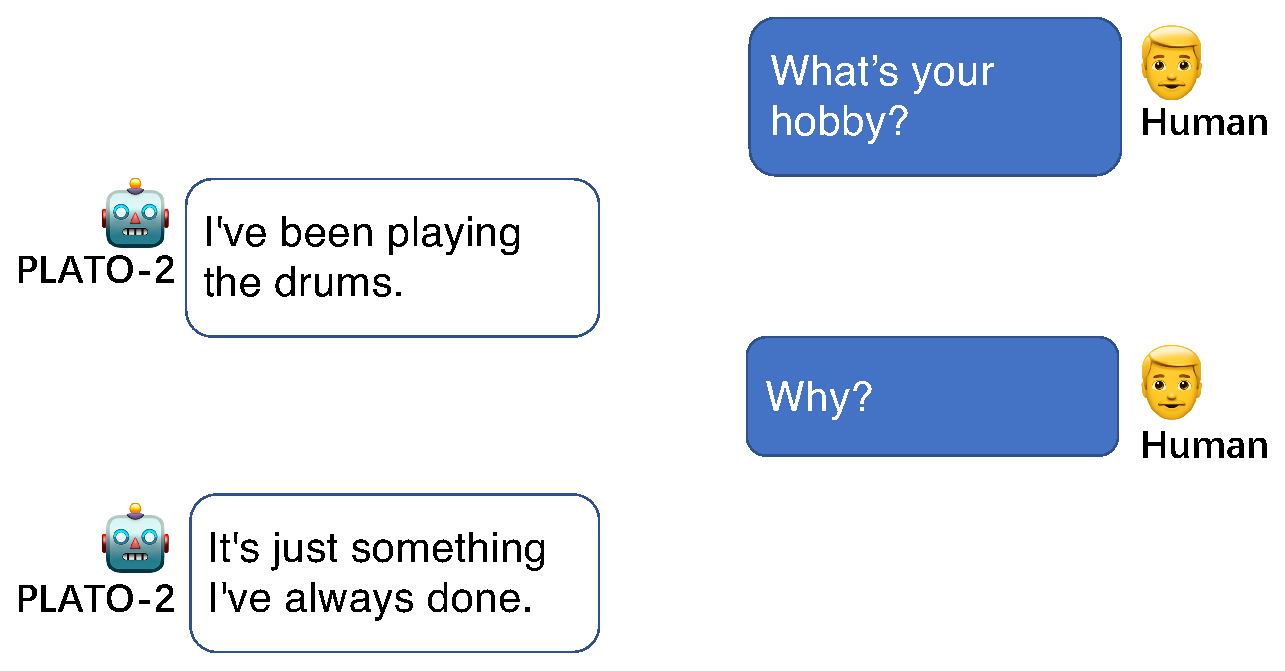
\includegraphics[width=.8\linewidth]{crop1.eps}  
  \caption{A small fragment of conversation between human and bot}
  \label{fig:sub-first}
\end{subfigure}
\begin{subfigure}{0.5\textwidth}
  \centering
  % include second image
  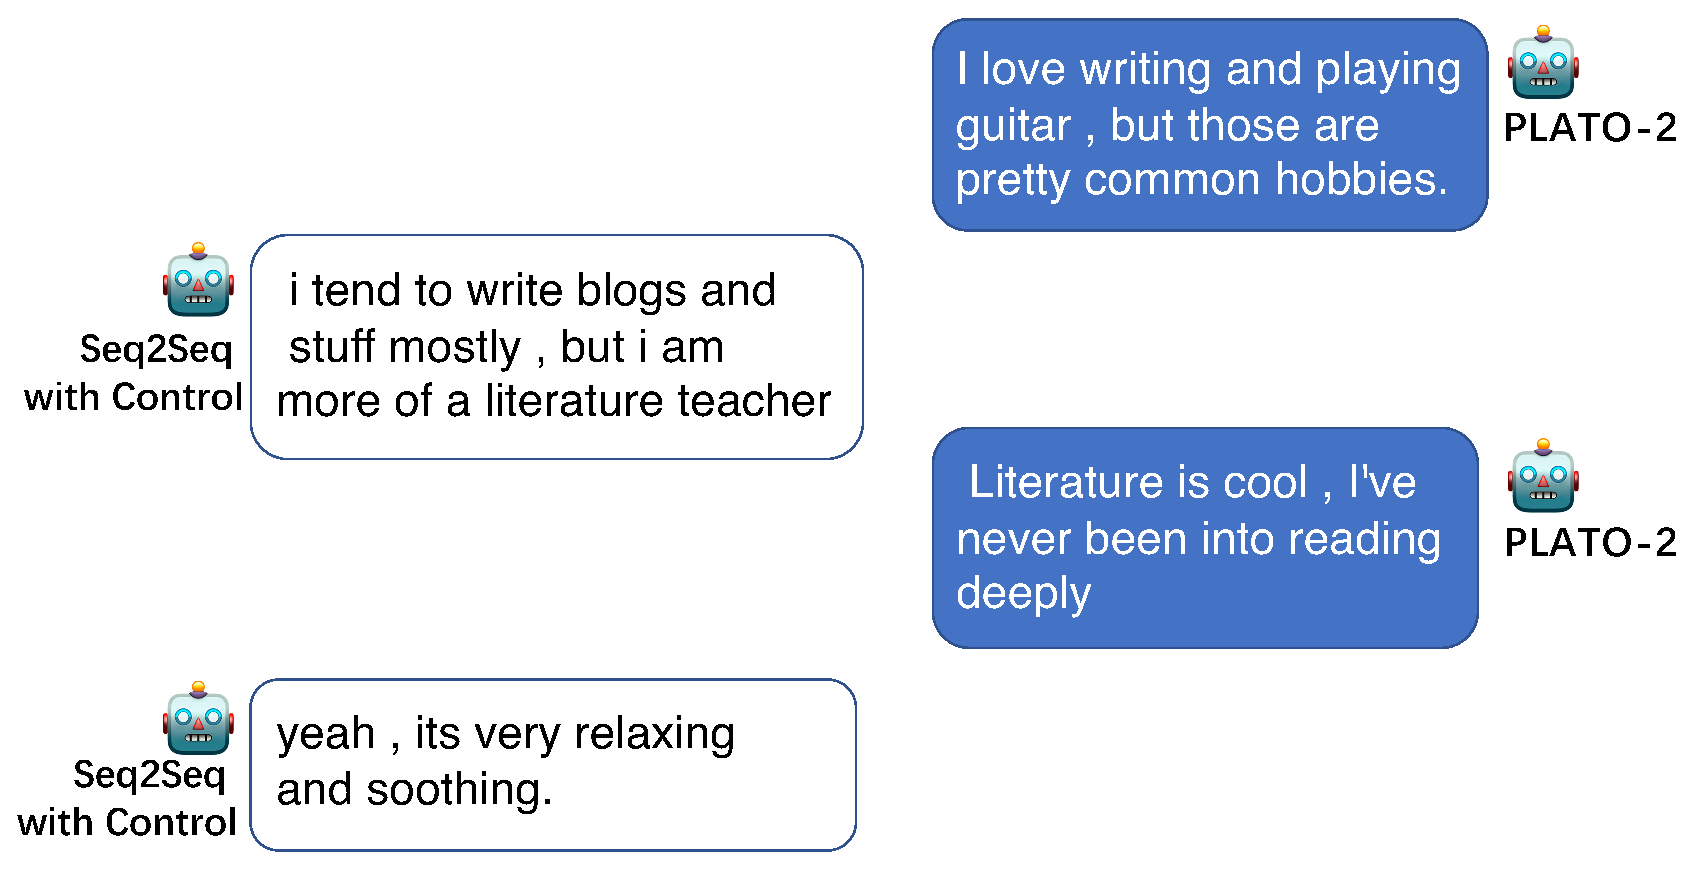
\includegraphics[width=\linewidth]{crop2.eps}  
  \caption{A small fragment of conversation between bot and bot% \KZ{crop the margins
%in this pic or use eps for both.} 
}
  \label{fig:sub-second}
\end{subfigure}
\caption{Small fragments from the chat logs between humans-bot and bot-bot}
\label{fig:two convs}
\end{figure}

Our framework consists of two components: \textit{competition} and 
\textit{scoring}, which may happen simultaneously. The competition is modeled
after most sport tournaments such as soccer or ping pong. 
There are three levels of competitions: 
game-level, match-level and tournament-level. 
Each match consists of several games. During a game, two bots will converse 
freely with each other and a virtual judge will score their performances according to
a group of criteria such as consistency and fluency, etc. 
%As an example like \figref{fig:example} shows, 
%Bot $A$ will be 
%penalized twice for repeating while Bot $B$ will be penalized once for 
%contradicting itself. In addition to the penalty, 
%a bonus point is rewarded to $A$
%who shows to produce relevant response with long term memory. 
%\KZ{Do we still have this as a criterion?}
%However, the specific bonus and penalty settings may vary 
%depending on the domain and scenarios that the experiment is 
%set in. 

%\begin{figure}[th!]
%	\centering
%	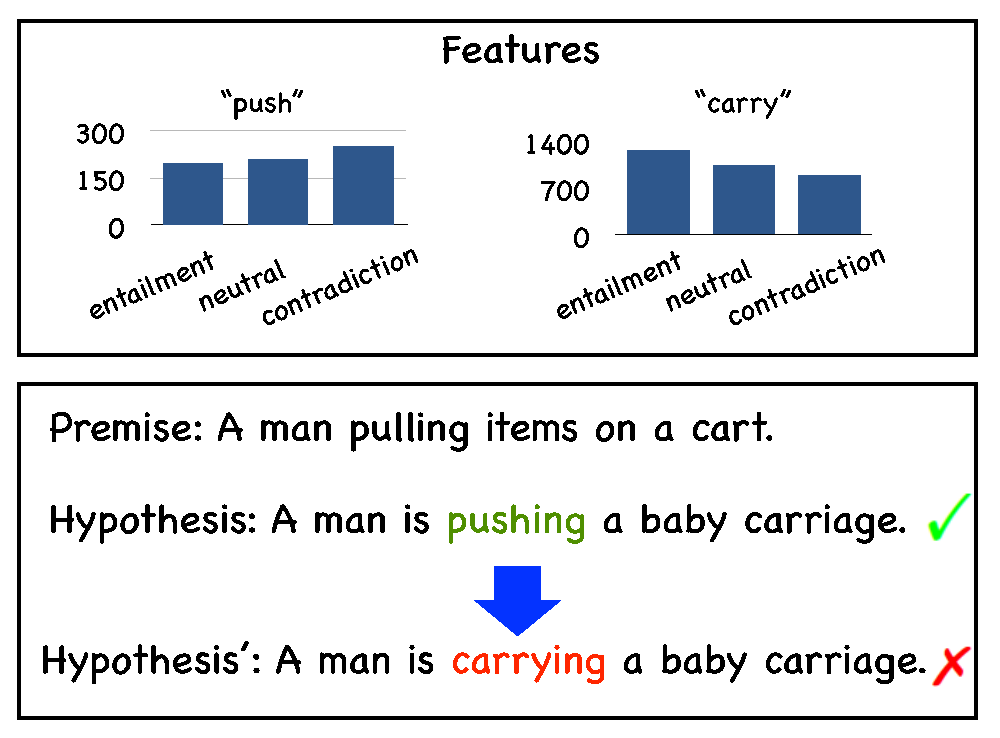
\includegraphics[width=0.95\columnwidth]{example.eps}
%	\caption{A chat snippet between two bots.}
%	\label{fig:example}
%\end{figure}

The main contributions of this paper are:
\begin{itemize}
\item We propose the first interactive evaluation framework for chatbots which
is based solely on bot-to-bot conversations and modeled after sports competitions (\secref{sec:competition}).
\item  The entire scoring process is fully automated and efficient. 
The system can rank seven bots in three minutes on average.
(\secref{sec:scoring}, \secref{sec:time}).
\item  Our experiments show that our scoring system closely tracks the 
human evaluation results. Preliminary results also show
that our evaluation system outperforms 
several recent strong baseline evaluation systems (\secref{sec:main}).
\item %We demonstrate the improvements in efficiency 
%using direct chat logs between bots.
We show that the chats between bots are impressively informative, 
even richer than the chats between humans and bots.
This suggests some possible directions to improve 
the capabilities of bots in the future.
(e.g., by having them learn from each other)  (\secref{sec:diversity})
\end{itemize}

\section{Task Definition}
We formulate our recommendation problem as the sequential recommendation or next item prediction. Assume that each user $u$ has a corresponding interaction sequence $S_u$, which can be represented as \[S_u=\{(x_1,c_1,T_1),(x_2,c_2,T_2),...,(x_T,c_T,T_T)\},\] where $x_j$ denotes the $j$-th news articles that user $u$ interacts with, and $c_j$ denotes the context embedding vectors of the corresponding articles, and $T_j$ denotes the intra-session temporal information of the corresponding interactions. Noted that each user $u$ only appear once, $S_u$ is corresponding to different sessions. Each $S_u$ starts at time $T_u$.

The intra-session temporal information $T_j$ contains two part. One is the time of $j$-th interaction $Tc_j$, which means the time user $u$ \textit{clicks} the $j$-th article and reflects it's position in $S_u$. The other is the \textit{publish} time of $j$-th article $Tp_j$, reflecting the refreshness of it. The $T_u$ reflects the inter-session temporal information because sessions with close start time are more related to each other.

Given a target user $u$ with her sequential of interactive behaviors over items $S_u$, our personalized next-item recommendation task is to predict $x_{T+1}$ that the target user $u$ is most likely to access in his/her next visit. Noted that the long term history of user $u$ is invisible, and we're supposed to predict $x_{T+1}$ in real-time right away after sequential of interactive behaviors from $x_1$ to $x_T$. The whole procedure is depicted in \figref{fig:representation}.


\section{Approach}
\label{sec:approach}
In this section, we first introduce the general framework of ChatMatch, which is modeled as
a sport tournament, then discuss some possible scoring functions that can be used by
the virtual judges in these competitions.

%Our whole evaluation framework consists of competition and scoring at three different levels. 
%The game level is at the bottom 
%and is played between two players. 
%Then comes the match level.
%To ensure the fairness of the game, 
%two games will be played between every two robots, 
%with each side starting a conversation.
%The result of two games determines the outcome of a match. 
%The tournament level is at the top
% and is composed of matches among different pairs of players. 

\subsection{Competition Protocol}
\label{sec:competition}
The competition takes place, from top to bottom, at tournament, match and
game levels.

\subsection*{Tournament Rules}
%\KZ{Give an overview of the how the tournament is run.}
We adopt a double round-robin 
sports tournament, where all bots participating in the competition 
converse directly with each other twice.
This is better than a knock-out system because it assesses a bot's ability to
deal with both strong and weak bots.
%For example, whether with weaker bots will induce them to make more mistakes or  how stronger bots will motivate their performance.
If we have $n$ chatbots players in our tournament, 
there will be $n\times (n-1) $ games in total.

\subsection*{Match Rules}
%\KZ{Talk about how the matches are administered. Just the procedure only.}
There are two chatbots competing in a single match. 
Each match consists of two games,
 started by a different bot. 
If we have $n$ bots in our tournaments, there 
will be ${n \choose 2}$ matches in total. 

\subsection*{Game Rules}
%\KZ{The procedure of the game. How each game is started and stopped.}
Each game is started by a player whose first utterance is provided by 
the system. The choice of the first utterance can be different 
depending on the domain of the bots and the ability we want to 
rank about the bots. For example, if we want to test 
the ability on movies, we can set a movie-related 
first utterance. 

During a game, there might be different ways to 
end the conversation. We can set a fixed number of exchanges 
or a terminating condition such as whether a bot makes a fatal error
or whether a certain score is reached.

\begin{table*}[th]
\centering
\scriptsize
\begin{tabular}{c|l|l}
%\hline
\toprule
\textbf{Dimension} & \textbf{Definition} &\textbf{Approach} \\ \midrule
Fluency  & Responses are fluent and natural.& Sentence perplexity. \\
Knowledge & Responses indicate the bot has the knowledge. & The number of times the bot expresses its ignorance to a question.\\
Proactivity & Responses actively proceed the conversation.&The number of times the bot raises a question. \\
Specificity & Responses are not generic.&The average of Distinct-1 and Distinct-2 \citep{li2015diversity}.\\
Diversity &Responses which are diverse and non-repetitive. &Repetition detection following the function in \algoref{algo:rep}. \\
Consistency &Responses do not contradict chat history. &Detect inconsistent questions following the function in \algoref{algo:inconsist}\\
Relevance & Responses are related to current context.& Ability to catch the relevant concept in chat history defined in \algoref{algo:bonus}. \\
\bottomrule
\end{tabular}
\caption{Seven evaluation dimensions.}
\label{tab:methods}
\end{table*}


\subsection{Scoring}
\label{sec:scoring}
\subsection*{Game-level Scoring}
%\KZ{Define a few functions: one to catch repeating, one to chat contradiction and one to catch long term memory.}

%Here we define the rules for recording points in one game between two bots. 
Inspired by \citet{finch2020towards}, 
we score each turn based on seven aspects of rules 
concerning \textit{consistency}, \textit{fluency}, \textit{knowledge}, \textit{specificity}, 
\textit{diversity}, \textit{relevance} and \textit{proactivity}. 
%As these seven metrics present a high level of 
%overlap among all distinct evaluation metrics used 
%during different process of human evaluation,
%we believe the combination of these seven distinct dimensions will be reliable. 
Finally, we sum up the scores for each bot for all the turns.
\tabref{tab:methods} documents the definition of these dimensions, which can all be scored
automatically.

%After finishing the calculation of the bonus and penalty scores for each turn, we obtain the scores of the two bots in a game with weighted sum according to \eqnref{eq:sum-up}

%\begin{equation}
%S(bot) = \sum_t - c\times C(t)  - r \times R(t) + b \times B(t)
%\label{eq:sum-up}
%\end{equation}
%$S$ denotes the total score gained by a bot for a game.
\begin{figure}[th]
        \centering
        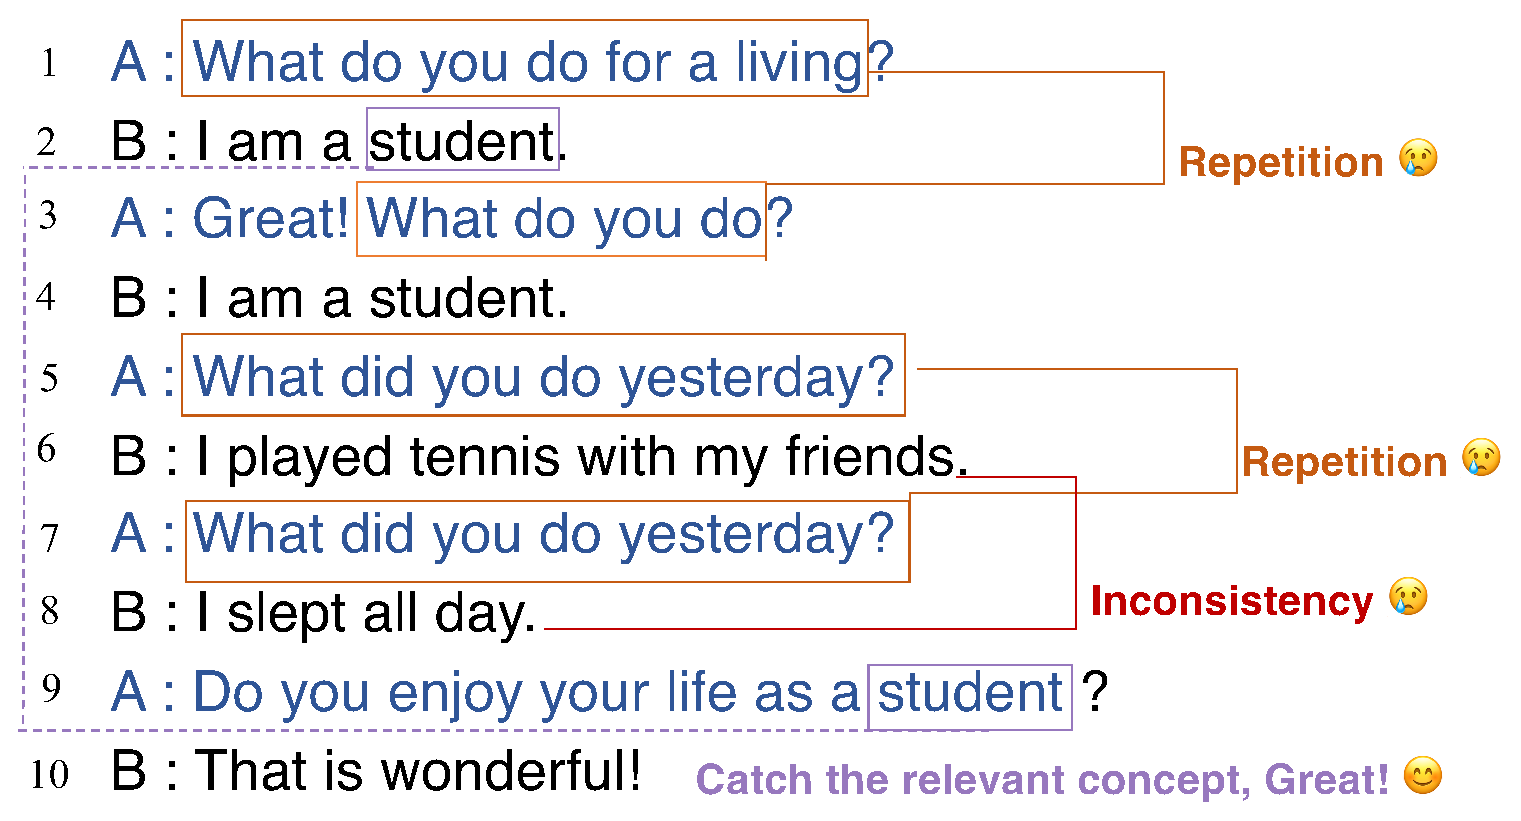
\includegraphics[width=0.95\columnwidth]{example2.eps}
        \caption{A chat snippet between two bots.}
        \label{fig:example}
\end{figure}

Fluency, Knowledge, Proactivity and Specificity are scored for each turn separately
and aggregated at the end of the conversation.
Detection for diversity, consistency and relevance are more involved and are explained
using \figref{fig:example}. 

As for diversity, at each turn $t$, we first check if there exists any repetitive question.  
We can easily find turn 3 and turn 7 repeated turn 1 and turn 5 
respectively. They will then be penalized one point for repetition. 
Repetition is not penalized if the previous turn is already 
marked as a repetitive question. For example, in \figref{fig:example}, 
although turn 4 is considered a repetition of turn 2,  
we are not going to penalize it as turn 3 is a repetitive question. 

The detection of inconsistency is always triggered after the detection of repeated questions. 
If the answers to the same questions are different, we will penalize the current turn, 
such as turn 8 in \figref{fig:example}.

We decide a repetition or an inconsistency by calculating the similarity of the two turns. 
We use a similarity function to complete the calculations, which we will 
discuss in \secref{sec:experiment}. The actual diversity and consistency scores
are the negation from the amount of repetition and inconsistency.

Relevance is assessed as a bonus to reward
a bot if it is able to memorize the important relevant concepts that have shown up 
before in the conversation. We sort the concepts that have shown up in 
chat history by their IDF scores. For example, in turn 9, $A$ 
mentions the concept word ``student'' presented by $B$ in turn 2. With this
turn, $A$ will win a bonus point.


The algorithms and notations for computing diviersty, consistency and relevance are included
in \tabref{tab:functions}, \algoref{algo:rep}, \algoref{algo:inconsist}, and \algoref{algo:bonus}. 

\begin{table}[th]
\centering
\small
\begin{tabular}{c|l}
%\hline
\toprule
\textbf{Notation} & \textbf{Description} \\ \midrule
$t$ & Current turn \\
$H(t)$  &  a list of history turns prior to $t$ \\
$Sim(x,y)$ & similarity between two turns $x$ and $y$ \\
$\sigma_r$ & Threshold for detecting repetition \\
$\sigma_c$ & Threshold for detecting consistency \\
$r$ & Weight for repetition \\
$c$ & Weight for inconsistency \\
$b$ & Weight for bonus \\
$d$ & Min distance between consecutive mentions \\
IDF list & List of lemma in chatlog sorted by IDF\\
$p$ & Percentage of important lemmas in IDF list\\
$R(t)$ &  Repetition penalty for turn $t$ \\
$C(t)$ &  Inconsistency penalty for turn $t$ \\ 
$B(t)$ &  Memory bonus for turn $t$ \\
$Rep(t)$ & A list of repeated turns for turn $t$ \\  
\bottomrule
\end{tabular}
\caption{
Functions and variables in algorithms.}
\label{tab:functions}
\end{table}

\begin{algorithm}[th]
\small
\caption{Scoring for Diversity}
\label{algo:rep}
\hspace*{0.02in} {\bf Input:}
 $t$, $H$, $Sim$, $\sigma_{r}$
; \hspace*{0.02in} {\bf Output: } 
 $R$;
\begin{algorithmic}[1]
\State //Starting to detect repetition
\For {$u$ in $H(t)$}
	\If {$Sim(t,u) \geq \sigma_{r}$}
		\State Add $u$ to $Rep(t)$
	\EndIf
\EndFor
    \If{$len(Rep(t))\geq 0$}
        \If{$t$ is a question and We can find a question in $Rep(t)$}
        \State $ R(t) \leftarrow  R(t) + 1$ 
        \Else
        \If {the previous turn of $t$ is not a repetitive question}
        \State $R(t)) \leftarrow R(t) + 1$ 
        \EndIf
        \EndIf
    \EndIf
\end{algorithmic}
\end{algorithm}


\begin{algorithm}[th]
\small
\caption{Scoring for Consistency}
\label{algo:inconsist}
\hspace*{0.02in} {\bf Input:}
$t$, $H$, $Sim$, $\sigma_{c}$
; \hspace*{0.02in} {\bf Output:  } 
 $C$;
\begin{algorithmic}[1]
\State // Inconsistency detection
 \If {previous turn of $p$ is a repetitive question} 
   \If{ the response $res$ to the question repeated by turn $p$ contradicts turn $i$ with $Sim(t, res) \leq \sigma_{c}$ }
    \State $C(t) \leftarrow C(t) + 1$
   \EndIf
  \EndIf
\end{algorithmic}
\end{algorithm}

\begin{algorithm}[th]
\small
\caption{Scoring for Relevance}
\label{algo:bonus}
\hspace*{0.02in} {\bf Input:}
$t$, $p$, $d$
; \hspace*{0.02in} {\bf Output:  } 
$B$;
\begin{algorithmic}[1]
\State // Assessing the ability of catching relevant concepts\\
$B(t) \leftarrow 0$
\For {all tokens $tk$ in current turn $t$}
 \If {$t$ - previous occurrence turn of $tk > d$ and $tk$ in the top $p\%$ of the IDF list of all tokens in the dialogue} 
   \State $B(t) \leftarrow 1$
  \EndIf
 \EndFor
\end{algorithmic}
\end{algorithm}

At the end of each game, each bot gets seven scores, one for each dimension.  
After pairwise comparison on individual dimension, a bot gains one point for win and zero point for a tie or lose.
The final score of each bot is determined by the sum of their individual scores.
%\KZ{Are these scores positive or negative? Comparable between bots?}

\subsubsection*{Match-level Scoring}
%\KZ{Use an equation to compute the final scores?}
One match which consists of two games, each started with a different bot, 
decides winning or losing between two bots.
For match-level scoring, we mimic the scoring rules of soccer tournament. 
For each match, $W$ points for the winner,  
$T$ points for a tie and 
$L$ points for the loser.
The value of $W$, $T$ and $L$ will be discussed in \secref{sec:ablation}. 

%\KZ{At the match level, we need to consider different starting context for the bots? I think we should present a few options for the reader and say that we are limited to these.}

\subsubsection*{Tournament-level Scoring}
%\KZ{Use an equation to compute the final scores?}
We count the points by simply summing up their scores gained in every match. Currently, several bots with the same final rank are tolerated. For future study, it's possible to mimic more detailed rules presented in sports match such as determine their ranking based on their win-loss relationship in the match between them.  
If they are still tied, we could propose an “overtime” for these two bots, one human judge may observe their performance and then make the decision of the game.

\section{Injecting Pre-processed Features} 
\label{sec:feature}
To pursue better dialogue understanding and reasoning, different features either designed by experts back on linguistic knowledge or engineered with observations are proposed to simulate the human comprehension process.
Recognizing these features is not only independent dialogue analysis 
tasks but also critical enablers for downstream applications. 
A subset of these features has been proved helpful for dialogue summarization by extracting from $D$ explicitly and injecting it into the vanilla model.
We group different features into two sub-categories by their scopes:
\begin{itemize}
	\item \textbf{Intra-utterance features} are features within an utterance or for an individual utterance.
	\item \textbf{Inter-utterance features} are features connecting or distinguishing multiple utterances.
\end{itemize}



\subsection{Intra-Utterance Features}

We divide the intra-utterance features into three groups: word-level, 
phrase-level or utterance-level.


\subsubsection{Word-level}
Word-level intra-utterance features include TF-IDF weights, Part-of-speech (POS) tags, and named entity tags.

The \textbf{TF-IDF weight} is a well-known statistical feature for each word, signifying its importance in the whole corpus. 
Term-frequency (TF) is the number of word occurrences in a dialogue or an utterance divided by the number of words. Inverse-document-frequency (IDF) refers to the logarithm of the number of dialogues or utterances divided by the number of them containing the word.
Each dialogue or utterance can be represented by a vocabulary-sized TF-IDF weight vector, where each element is the product of TF and IDF. 
In early work, \citet{murray2005extractive} used such utterance vectors as features for classifiers to find important utterances.
This feature is still prevalent in constructing better prompts for the summary generation with large language models~\cite{prodan2021prompt}.


\textbf{POS tags} and \textbf{named entity tags} are linguistic labels assigned for each word. POS tags represent grammatical properties, including nouns, verbs, adjectives, etc. Named entity tags belong to pre-defined categories such as person names, organizations, and locations. Both of them are easily labeled by well-known NLP packages such as NLTK and Spacy, 
and can be assigned to summaries in the training set~\cite{OyaMCN14,singla2017spoken}, to generate summary templates for abstractive text summarization without neural models. 
\citet{zhu2020end} trained two embedding matrices for both tags and concatenated them with word embeddings as part of the embedding layer for the model, i.e.
$x_i^t = [e_i^t;POS_i^t;ENT_i^t]$. 
$e_i^t$, $POS_i^t$, and $ENT_i^t$ are the word embedding, POS embedding, and named entity embedding for $x_i^t$, respectively. These features, which were also adopted by \citet{qi2021improving} in the same way, work for hierarchical models trained from scratch on this task and 
help with language understanding and entity recognition. 
However, the probing tests indicated that pre-trained 
language models have already captured both features well 
implicitly~\cite{tenney2018you}, and the two are no longer 
needed. 

\subsubsection{Phrase-level}
Intra-utterance features here have key phrases/words and negation scopes.
 
\textbf{Key phrases/words} emphasize salient 
n-grams in the original dialogue, which can help with the information scattering challenge and lead to more informative summaries. 
The definition of key phrases varies.
\citet{wu2021controllable} regarded the longest common sub-sequence (LCS) between each candidate phrase, extracted from $D$ first using a trained constituency parser, and $Y$ as key phrases. 
The LCSs are concatenated into a sketch, 
which is prefixed to $Y$ as a weakly 
supervised signal for the summary generation. 
Similarly, \citet{zou2021topic} proposed that words that appear both 
in $D$ and $Y$ are salient or informative topic words, i.e., another kind of keywords. 
They used an extension of the Neural Topic Model (NTM)~\cite{miao2017discovering} to learn the word-saliency correspondences. 
Then, input utterances are converted to topic representations by the saliency-aware NTM and further incorporated into Transformer Decoder layers for a better extractor-abstractor two-stage summarizer.
Differently, \citet{feng2021language} regarded unpredictable words by DialoGPT as keywords since they assumed that highly informative words could not be predicted. 
They appended all extracted keywords at the end of $X$ as inputs to the summarization model. 


The \textbf{negation scope} is also a set of consecutive words  
reflecting denied contents in utterances. \citet{chen2020multi} pointed out that negations are challenging for dialogues. With that in mind, \citet{khalifa2021bag} trained a Roberta model on CD-SCO dataset~\cite{morante2012sem} for negation scope prediction, which labels the beginning and end positions of sentences' negation scopes in $D$ with designated special tokens. Unfortunately, inputting such labeled $D$ to the model hurt the performance according to their experiment results. Negations are of great importance in task-oriented scenarios for generating accurate facts, such as realizing the patient's confirmation or negation of a symptom in a medical care conversation. \citet{joshi2020dr} proposed using an additional binary vector to label each $x_i$ based on a set of manually-curated negative unigrams, and to modify the cross-attention distribution. Besides, they extended the vocabulary with a special token `[NO]' and 
learned when to generate it by formulating the probability distribution over extended vocabulary, similarly to~\citet{see2017get}. The results showed reductions in coherency despite capturing negations.


\subsubsection{Utterance-level}
Speakers or roles, redundancies, user intents, and dialogue acts are utterance-level intra-utterance features. 
Domain knowledge is another kind of intra-utterance feature. It lies across phrase-level to utterance-level depending on specific circumstances. 

\textbf{Speaker} or \textbf{role} is a naturally provided ``label'' for each dialogue utterance. 
Since the general default input to models is the concatenation of all of 
the utterances into a sequence of tokens, each speaker or role token $s_t$ 
is encoded just like any other content token $w_i^t$~\cite{chen2020multi,feng2021language}. Thus, the speaker or role 
information is likely ignored or misunderstood, especially by language models pre-trained 
on common crawled texts. 
For a better utilization of speaker information, \citet{lei2021hierarchical} introduced Speaker-Aware Self-Attention made up of Self-Self Attention and Self-Others Attention, which only considered whether utterances were from the same speaker. This structured feature is also 
adopted in~\cite{lei2021finer}.
In addition, the number of speakers is used as a feature for 
finding similar dialogues in the training set by \citet{prodan2021prompt}.
In TDS, the number of roles is always fixed in a specific scenario, although the speakers are various among dialogue sessions.
\cite{yang2022tanet} modified the input with template ``\{\textit{speaker}\} of role \{\textit{role}\} said: \{\textit{utterance}\}''.
Other previous work only focuses on modeling roles, reflecting functional information bias in utterances. 
The cheapest way is to represent each role with a dense vector $r_t$ which is either obtained by randomly initialized trainable vectors~\cite{zhu2020end,duan2019legal,qi2021improving,gan2021inspectional,asi2022end} or a small trainable neural network~\cite{song2020summarizing}. This vector is further concatenated, summed up, or fused by non-linear layers with input embeddings $e_i^t$ or utterance-level representations $h_t^u$ in summarization models. 
There are also works that capture such features by different sets of model parameters for different roles~\cite{zou2021topic,zhang2020unsupervised,yuan2019scaffolds}. More complicated methods that regard speakers or roles as graph nodes beyond the utterance-level are in \secref{sec:graphs}.


Since dialogue utterances are mixed with backchanneling or repetitive confirmations~\cite{sacks1978simplest}, \textbf{redundancy} is also a significant 
feature where each utterance is either preserved or removed. 
\citet{murray2005extractive} and \citet{zechner2002automatic} regarded 
utterances similar to the previous ones as redundant by calculating 
the cosine similarity between two sentence vectors 
computed using TF-IDF features. {Then, the remaining utterances can be regarded as a summary}.
Different from previous work calculating similarities between individual utterances,
\citet{feng2021language} brought the context into consideration which calculated similarities on the dialogue level.
Utterance representations $h_t^u$ are collected by inputting the whole dialogue into DialoGPT~\cite{zhang2020dialogpt}. 
Then, they assume that if adding an utterance $u_{t+1}$ to the 
previous history $\{u_1, ..., u_t\}$ doesn't result in a big difference 
between the context representation $h_t^u$ and $h_{t+1}^u$, 
$u_{t+1}$ will be regarded as a redundant utterance. 
Such features will be added as part of the dialogue input with special tokens. 
\citet{wu2021controllable} regarded non-factual utterances 
such as chit-chats and greetings as redundancies, and removed them by a sentence compression method with neural content selection for their summary sketch construction.

Another group of utterance-level features is matching each utterance with 
a label from a pre-defined multi-label set. \citet{wu2021controllable} defined 
a list of interrogative pronoun category to encode the \textbf{user intent}, including \textit{WHY}, \textit{WHAT}, \textit{WHERE}, 
\textit{WHEN}, \textit{CONFIRM} and \textit{ABSTAIN}. 
Each utterance is labeled by a few heuristics and these user intents are combined with the keywords and redundancies mentioned above as a sketch prefixed to the summary output.
This definition is different from the so-called user intent in task-oriented dialogue systems, while the latter can be used for TDS and will be discussed in domain ontologies in \secref{sec:graphs}.

A more widely-accepted label set is \textbf{dialogue act}, which is defined as the functional unit used by speakers to change the context~\cite{bunt1994context} and has been used for different goals~\cite{kumar2018dialogue, oraby2017may}. The whole dialogue act taxonomy, including dialogue assess, inform, offer, etc., is tailored for different scenarios. For example, only 15 kinds of dialogue are labeled in the meeting summarization corpus AMI~\cite{carletta2005ami} 
while the total number of categories is 42~\cite{stolcke2000dialogue}. \citet{goo2018abstractive} explicitly modeled the relationships between dialogue acts 
and the summary by training the dialogue act labeling task and 
abstractive summarization task jointly. 
\citet{di2020da} further added the dialogue act information as a contextualized 
weight to $h_t^u$. These labels are required from human annotators. 

\textbf{Commonsense knowledge} generated by widely-used generative commonsense model PARA-COMET~\cite{gabriel2021paragraph} is considered in~\cite{kim2022mind}. PARA-COMET takes dialogue history with the target utterance or a summary sentence as input and outputs short phrases for each of the 5 relation types, which are strongly correlated with speakers' intentions and the hidden knowledge, such as ``XINTENT'' and ``XREACT''. The generated knowledge is concatenated with each utterance as input and is used as an additional generation target in a dual-decoder setting.

In addition, \textbf{domain knowledge} plays an important role in TDS. 
\citet{koay2020meet} showed that the existence of 
terms affects summarization performance substantially. 
Such knowledge is considered as intra-utterance features in previous work.
\citet{joshi2020dr} leveraged a compendium of medical concepts for 
medical conversation summarization. They incorporated domain knowledge at 
the phrase level by simply encoding the presence of medical concepts, which 
are both in the source and the reference. The corresponding one-hot vectors 
affect the attention distribution by the weighted sum with contextualized 
hidden states $H$ for each word only during training, like the teacher forcing strategy.
\citet{gan2021inspectional} defined a number of domain aspects, and labeled text spans manually in $D$ and $S$. Auxiliary classification tasks of these aspects help generate more readable summaries covering important in-domain contents. 
Differently, \citet{duan2019legal} incorporated their legal 
knowledge for each utterance. This is because their legal knowledge graph 
(LKG) depicts the legal judge requirements for different cases rather than a dictionary to look up, and each node represents a judicial factor 
requiring semantic analysis beyond the word level. A series of graph 
knowledge mining approaches were adopted to seek relevant knowledge w.r.t. 
each utterance $u_t$, and the legal knowledge embedding was added 
to the sentence embedding $h_t^u$ for further encoding.
 

\subsection{Inter-Utterance Features}\label{sec:interutt}

As dialogue utterances are highly dependent, information transitions among utterances are of great importance for dialogue context understanding. 
Multiple inter-utterance features show up for more efficient and 
effective dialogue summarization, which can be categorized into 
two sub-categories:
\begin{itemize}
	\item \textbf{Partitions} refer to extracting or segmenting the whole dialogue into relatively independent partitions. Information within each partition is more concentrated with fewer distractions for the summary generation. Meanwhile, these features reduce the requirements on GPU memory with shorter input lengths, which are especially preferred for long dialogue summarization.
	\item \textbf{Graphs} refer to extracting key information and relations from utterances to construct graphs, serving as a complement to the dialogue. These features are designed to help the summarization model understand the inherent dialogue structure.
\end{itemize}


\subsubsection{Partitions} 

There are two types of partitions.
One is to cut the dialogue into a sequence of $K$ consecutive segments $\{S_k|_{k=1}^K\}$ with or without overlaps, i.e., $|D|\leq|S_1| + ... + |S_K|$, where $|\cdot|$ counts the number of utterances. Representative features under this category are as follows.


\textbf{Topic transition} is important for dialogues where speakers turn to focus on different topics. Consecutive utterances that focus on the same topic constitute a topic segment, which should meet three criteria\cite{arguello2006topic}, including being reproducible, not relying heavily on task-related knowledge,  and being grounded in discourse structure.
Some previous works annotate this feature when constructing datasets such as \citet{carletta2005ami} and \citet{janin2003icsi}. 
\citet{di2020da} took advantage of such labeled information during decoding.
Others collected such features by rules or algorithms.
\citet{asi2022end} adopted the text segmentation idea from~\citet{alemi2015text} and broke the long dialogue into semantically coherent segments by word embeddings.
\citet{liu2019topic} regarded different symptoms as different topics in medical dialogues and detected the boundaries by heuristics.
To alleviate human annotation burdens, unsupervised topic segmentation methods are adopted. \citet{chen2020multi} used the classic segmentation algorithm C99~\cite{choi2000advances} based on inter-utterance similarities, where utterance representations were encoded by Sentence-BERT~\cite{reimers2019sentence}. \citet{feng2021language} regarded sentences that are difficult to be generated based on the dialogue context to be the starting point of a new topic. Thus, sentences with the highest losses calculated based on DialoGPT are marked.
However, the window size and std coefficient for C99 algorithm in %~\cite{choi2000advances} 
\citet{chen2020multi} and percentage of unpredictable utterances in \citet{feng2021language} are still hyper-parameters that need assigning by humans.
Among these works, some models use topic transitions as prior knowledge and input to summarisation models. They either add special tokens to dialogue inputs~\cite{chen2020multi,feng2021language}, add interval segment embeddings, such as $\{t_a, t_a, t_b, t_b, t_b, t_a,...\}$ for each utterance~\cite{qi2021improving}, or guide the model on learning segment-level topic representations $h_k^s$ based on utterance representations $h_t^u$~\cite{zheng2020abstractive}.
Others adjust their RNN-based models to predict topic segmentation first and do summarization based on the predicted segments~\cite{liu2019topic,li2019keep}, either with or without using additional supervised topic labels for computing the segmentation training loss. 

Multi-view~\cite{chen2020multi} describes \textbf{conversation stages}~\cite{althoff2016large} from a conversation progression perspective. They assumed that each dialogue contained $4$ hidden stages, which were interpreted as ``openings$\rightarrow$intentions$\rightarrow$discussions$\rightarrow$conclusions'', and annotated with an HMM conversation model. In their approach, both the preceding topic view and such stage view are labeled on dialogues with a separating token ``|'', encoded with two encoders sharing parameters and guided the Transformer decoder in BART with additional multi-view attention layers. 

There also exists a simple \textbf{sliding-window} based approach that regards window-sized consecutive utterances as a snippet and collects snippets with different stride sizes.
On the one hand, it can be used to deal with long dialogues. Sub-summaries are generated for each snippet and merged to get the final summary.
Most works regarded the window size and the stride size as two constants~\cite{koay2021sliding,liu2021topic,zhang2021leveraging,zhang2021summ},
while \citet{liu2021dynamic} adopted a dynamic stride size which predicts the stride size by generating the last covered utterance at the end of $Y'$.
\citet{koay2021sliding} generated abstractive summaries for each snippet by news summarization models as a coarse stage for finding the salient information.
On the other hand, pairs of (snippet, sub-summary) are augmented data for training better summarization models.
By calculating Rouge scores between reference sentences and snippets, 
the top-scored snippet is paired with the corresponding sentence~\cite{liu2021topic, zhang2021summ}.
Alternatively, multiple top-scored snippets can be merged as the corresponding input to the sentence~\cite{zhang2021leveraging} for the sub-summary generation. 
However, the gap between training and testing is that we don't know the oracle snippets since there is no reference summary during testing.
Therefore, each snippet was also considered to be paired with the whole summary~\cite{zhang2021leveraging,zhang2021summ}, but it leads to hallucination problems.
These constructed pairs can also be used with an auxiliary training objective~\cite{liu2021topic}, or as pseudo datasets for hierarchical summarization~\footnote{Hierarchical summarization means we do summarization, again and again, using the previously generated summaries as input to get more concise output. These models either share parameters~\cite{li2021hierarchical} or not~\cite{zhang2021leveraging,zhang2021summ} in each summarization loop.}.



The other is to \textbf{cluster utterances} or \textbf{extract utterances} into a single part or multiple parts $\{P_l|_{l=1}^{K'}\}$. In this way, outlier utterances or unextracted utterances will be discarded, i.e., $|D|>|P_1| + ... + |P_K'|$. Then, the abstractive summarization model is trained between the partitions and the reference summary. The whole process can be regarded as variants under the extractor-abstractor framework for document summarization~\cite{chen2018fast,liu2021keyword}. 

\citet{zou2021unsupervised} proposed to select topic utterances according to 
centrality and diversity\footnote{Centrality reflects the center of utterance clusters in the representation space. Diversity emphasizes diverse topics among selected utterances.} in an unsupervised manner. Each utterance with its surrounding utterances in a window size forms a topic segment.
\citet{zhong2021qmsum} extracted relevant spans given the query with the Locator model which is initialized by Pointer Network~\cite{vinyals2015pointer} or a hierarchical ranking-based model. 
Cluster2Sent by~\citet{krishna2021generating} extracted important utterances, clustered related utterances together and generated one summary sentence per cluster, resulting in semi-structured summaries suitable for clinical conversations. 
\citet{banerjee2015generating} and \citet{shang2018unsupervised} followed a similar procedure, i.e., (segmentation, extraction,  summarization) and (clustering, summarization) respectively.
The oracle spans are required to be labeled for supervised training of extractors or classifiers for most approaches, except that \citet{shang2018unsupervised} used K-means for utterance clustering in an unsupervised manner.
Generally, the partitions are concatenated as the input to summarization models~\cite{zhong2021qmsum}, or the generated summary of each segment is concatenated or ranked to form the final $\hat{Y}$~\cite{zou2021unsupervised,banerjee2015generating}.



\subsubsection{Graphs} 
\label{sec:graphs}

The intuition for constructing graphs is attributed to the divergent structure between dialogues and documents introduced in \secref{sec:divergence}. To capture the semantics among complicated and flexible utterances, a number of works constructed different types of graphs based on linguistic theories or observations and demonstrated improvements empirically. We group these graphs into three categories according to the type of 
nodes, i.e., being either a word, a phrase or an utterance. 

\textit{Word-level graphs} focus on finding the central words buried in the whole dialogue. Some works~\cite{OyaMCN14,banerjee2015generating,shang2018unsupervised,park2022unsupervised} parsed utterances together with or without summary templates using the Standford or NLTK packages. Words in the same form and the same POS tag or synonyms according to WordNet~\cite{MehdadCTN13} are regarded as a single node. The natural flow of text, parsed dependency relations and relations in WordNet are adopted to connect nodes, resulting in a directed \textbf{word graph}. It is used for unsupervised sentence compression by selecting paths covering nodes with high in-degree and out-degree without language models.

%Complex interactions within dialogues always make it hard for humans and models to associate speakers with correct events. At the same time, different surface forms of the same event and frequent coreferences increase the difficulty for the model to generate faithful summaries. 
The purpose for \textit{phrase-level graphs} is mainly to emphasize relations between important phrases.
\citet{liu2021coreference} and \citet{liu2021controllable} transferred document coreference resolution models~\cite{joshi2020spanbert,lee2018higher} to dialogues,  applied data post-processing with human-designed rules and finally constructed \textbf{coreference graphs} for dialogues. The nodes are mainly person names and pronouns, and the edges connect nodes belonging to the same mention cluster.
Based on the coreference results, \citet{chen2021structure} took advantage of information extraction system~\cite{angeli2015leveraging} and constructed an \textbf{action graph} with "WHO-DOING-WHAT" triples. 
\citet{zhao2021give} manually defined an undirected \textbf{semantic slot graph} based on NER and POS Tagging focusing on entities, verbs, and adjectives in texts, i.e., slot values. Edges in this graph represent the existence of dependency between slot values collected by a dependency parser tool.
More strictly defined ``domain-intent-slot-value'' tuples based on structured \textbf{domain ontologies} are marked in advance~\cite{yuan2019scaffolds,zhao2021todsum}. It is different from domain to domain, such as ``food, area'' slots 
for ``restaurant'' and ``leaveAt, arriveBy'' slot for ``taxi'' labeled in 
the MultiMOZ dataset~\cite{eric2019multiwoz}.
Ontologies in the medical domains containing clinical guidelines in 
``subject-predicate-object'' triples were introduced in~\citet{molennar2020healthcare}. Triples are extracted from $D$ and matched with the ontology to construct a patient medical graph for report generation.
Moreover, external commonsense \textbf{knowledge graphs}, 
such as ConceptNet~\cite{speer2012representing}, have been adopted to find the relations among speaker nodes, utterance nodes and knowledge nodes~\cite{feng2021incorporating}. 
%Their undirected graph use ``speaker-by'' edges connecting speaker nodes and utterance nodes and ``know-by'' edges connecting utterance nodes and knowledge nodes.



\textit{Utterance-level graphs} considering the relationship among utterances have been explored mainly in five ways. 
One is \textbf{discourse graph} mainly based on the SDRT theory~\cite{asher2003logics} which models the relationship between elementary discourse units (EDUs) with 16 types of relations for dialogues. Both \citet{chen2021structure} and \citet{feng2020dialogue} adopted this theory and regarded each utterance as an EDU. They labeled the dialogue based on a discourse parsing model~\cite{shi2019deep}. 
The former work used a directed discourse graph with utterances as nodes and discourse relations as edges.
Differently, the latter one transformed the directed discourse graph with the Levi graph transformation where both EDUs and relations are nodes in the graph with two types of edges, including default and reverse.  Self edges and global edges were also introduced to aggregate information in different levels of granularity.
\citet{ganesh2019restructuring} designed a set of discourse labels themselves and trained a simple CRF-based model for discourse labeling. Unfortunately, they haven't released the details so far.
\textbf{Dependency graph} can be regarded as a simplification of discourse graph since it only focuses on the ``reply-to'' relation among utterances.
The tree structure of a conversation is a kind of it and is adopted in~\cite{yang2022tanet} by modifying the self-attention into thread-aware attention which considers the distance between two utterances, and also proposing a thread prediction task to predict the historical utterances in the same thread for some sampled utterances.
Another one is \textbf{argument graph}~\cite{stede2016parallel} for identifying argumentative units, including claims and premises and constructing a structured representation. \citet{fabbri2021convosumm} did argument extraction with pretrained models~\cite{chakrabarty2019ampersand} and connected all of the arguments into a tree structure for each conversation by relationship type classification~\cite{mirko2020towards}. Such a graph not only helps to reason between arguments but also eliminates unnecessary content in dialogues. Similarly, \textbf{entailment graph}~\cite{MehdadCTN13} is used to identify important contents by entailment relations between utterances.
The fifth is \textbf{topic graph}. Usually, we regard the topic structure in dialogues as a linear structure as discussed above, but it can be hierarchical with subtopics~\cite{carletta2005ami, janin2003icsi} or non-linear structures since the same topic may be discussed back and forth~\cite{kim2019dynamic}.
\citet{lei2021finer} used ConceptNet to find the related words that indicate the connections among utterances under the same topic, capturing more flexible topic structures.


The graphs above are used in three ways. One is to convert the original dialogue into a narrative similar to documents by linearizing graphs and inputting to the basic summarization models~\cite{fabbri2021convosumm,ganesh2019restructuring}.
Second is to bring graph neural layers, such as Graph Attention Network~\cite{velivckovic2018graph} and Graph Convolutional Networks~\cite{kipf2016semi}. Such graph neural layer can be solely used as the encoder~\cite{feng2021incorporating}. It can also cooperate with the Transformer-based encoder-decoder models, either based on the encoder hidden states or injected into the Transformer layer in encoder~\cite{liu2021coreference} or decoder~\cite{chen2021structure}.
The rest modify attention heads in Transformer with constructed graphs from a model pruning perspective. \citet{liu2021coreference} replace attention heads containing the most coreference information with their coreference graph, while \citet{liu2023picking} replace underused heads with a similar graph.





\subsection{Multi-modal Features}

Humans live and communicate in a multi-modal world. As a result, multi-modal dialogue summarization is naturally expected. Even for virtual dialogues from TV shows or movies, character actions and environments in videos are important sources for humans to generate meaningful summaries. However, due to the difficulties of collecting multi-modal data in real life and the limited multi-modal datasets, this area remains to be researched. 
\textbf{Prosodic features} gained attention in early speech-related works.
\citet{murray2005extractive} collected the mean and standard deviation of the fundamental frequency, energy and duration features based on speech. %The features are collected at the word level and then averaged over the utterance.
With the marvelous automatic speech recognition (ASR) models, most works later only focused on transcripts and ignored such multi-modal features.
Besides, \textbf{visual focus of 
attention} {(VFOA)} feature from the meeting summarization scenarios 
has been introduced to highlight the importance of utterances~\cite{li2019keep}. 
It represents the interactions among speakers reflected by the focusing target that each participant looks at in every timestamp. They assumed that the longer a speaker was paid attention to by others, his or her utterance would be more important. Such orientation feature was converted into a vector by their VFOA detector framework and further concatenated to the utterance representations. 

\subsection{Summary and Opinions}

\begin{figure}
	\centering
	\includegraphics[scale=0.65]{fig/approach-feature.pdf}
	\caption{A summary of all features.}
	\label{fig:app-feature}
\end{figure}
The above features are summarized in 
Fig.~\ref{fig:app-feature} and mainly {injected into vanilla models} 
in three ways: 

\begin{itemize}
\item \textbf{Manipulating the input and output} by adding annotations or data reformulation. The former one adds additional tokens to the dialogue or summary to highlight the features, such as topic transition marks in the dialogue~\cite{chen2020multi} and key phrase prefixes of the summary~\cite{wu2021controllable}. This is suitable for features linearly buried in the texts. For the hierarchical or more complicated structures, researchers tend to reformulate the dialogue into different segments, especially for long dialogues~\cite{zhong2021qmsum,banerjee2015generating,shang2018unsupervised} or reordering utterances with graph features. For example,  \citet{fabbri2021convosumm} linearized the argument graph following a depth-first approach to fine-tune sequence-to-sequence models for summarization, and \citet{zhao2021todsum} linearized the dialogue states, i.e., slot-related labels, as a complement to $D$ with a bi-encoder model.



\item \textbf{Modifying the model architecture or hidden states} for learning inductive bias on known features. Embedding layers are always modified for word-level or phrase-level features indicating the binary or multi-class classification properties, including the POS embeddings in~\cite{zhu2020end} and medical concept embedding in~\cite{joshi2020dr}. Modifications on self-attentions and cross-attentions are used to merge multiple features and are also preferable to graph features. For instance, \citet{chen2020multi} modified the cross-attention layer for balancing and fusing hidden states of two kinds of labeled input from double encoders. \citet{lei2021hierarchical} changed the self-attention layer in the encoder with two speaker-aware attentions to highlight the information flow within the same speaker or among speakers. Different graph neural layers~\cite{feng2021incorporating,liu2021coreference,chen2021structure} are also introduced for capturing graph features.


\item \textbf{Adding additional training targets} means that features are regarded as a supervision output during training under multi-task learning and are ignored during inference. For example, \citet{goo2018abstractive}, \citet{li2019keep}, \citet{kim2022mind} used an additional decoder for dialogue act labeling, topic segmenting and commonsense knowledge generation, respectively.
\citet{yuan2019scaffolds} incorporated domain features by formulating domain classification as a multi-label binary classification problem for the whole $D$. All of them use utterance-level features to learn better encoder representations, which will lead to a high-quality summary.

\end{itemize}

The advantages and disadvantages of injecting pre-processed features are as follows:
\begin{itemize}
    \item[\Checkmark] Injecting pre-processed features as the mainstream research direction for dialogue summarization significantly improves the results compared with the basic summarization model. Features including negation scope, speaker/role, coreference graph, action graph and semantic slot graph pay more attention to generating consistent summaries, while most of the other features help to select valuable information for summarization.
    \item[\Checkmark] Such explicitly incorporated features are more interpretable to humans and can be manipulated for more controllable summaries. Different features can be selected and combined to promote the model performance in specific application scenarios.
        \item[\Checkmark] Features collected by labelers on other dialogue understanding tasks capture the essence of these tasks and also establish connections with various aspects of dialogue analysis.  Therefore, leveraging such features is a good way to alleviate the human labeling burden.
	\item[\XSolidBrush] Features are not transferable in different scenarios and some features are not compatible with each other, thus feature engineering is shown to be important.
	\item[\XSolidBrush] Labelers trained with other datasets are always out-of-domain compared to the targeting dialogue summarization scenario. Hyper-parameters introduced in labeling algorithms with these labelers need try and error for the domain transfer. 
	\item[\XSolidBrush] Error propagation exists in these dialogue summarization approaches. Incorrect features hinder the understanding of dialogues and lead to poor summaries. 
\end{itemize}
\section{Designing Self-supervised Tasks}
\label{sec:designselftasks}

To alleviate human labor and avoid error propagation, self-supervised 
tasks emerged, which leverage dialogue-summary pairs without additional 
labels.  We divide such tasks into three sub-categories:
\begin{itemize}
	\item \textbf{Denoising tasks} are designed for eliminating noises 
in the input or penalizing negatives.
	\item \textbf{Masking and recovering tasks} mean that parts of the input are masked and the masked tokens are required to be predicted.
	\item \textbf{Dialogue tasks} refer to response selection and generation for better dialogue understanding.
\end{itemize}


\subsection{Denoising Tasks}

Denoising tasks focus on adding
noises to the dialogue input or output and aims at generating concise summaries by filtering out the noisy information, resulting in more robust dialogue 
summarization models.
\citet{zou2021unsupervised} used the original dialogue as output and trained a denoising auto-encoder which is capable of doing content compression for unsupervised dialogue summarization.
Noising operations, which include fragment insertion, utterance replacement, and
content retention, are applied together on each sample.
For a utterance $u_t$ in $D$, \textbf{fragment insertion} means that randomly sampled 
word spans from $u_t$ is inserted to $u_t$ for lengthening the original 
sequence.
\textbf{Utterance replacement} is that $u_t$ is replaced by another utterance $u_{t'}$ in $D$ and \textbf{content retention} means that $u_t$ is unchanged. 
\citet{chen2021simple} augmented dialogue data by swapping, deletion, insertion 
and substitution on utterance level and used the corresponding summary as 
the output, resulting in more various dialogue inputs for training the summarization model. 
\textbf{Swapping} and \textbf{deletion} aim to perturb discourse relations by randomly swapping two utterances in $D$ or deleting some utterances.
\textbf{Insertion} includes inserting repeated utterances that are chosen from $D$ randomly and inserting utterances with specific dialogue acts such as self-talk or hedge from a pre-extracted set, mimicking interruptions in natural dialogues.
\textbf{Substitution} replaces the chosen utterances in $D$ by utterances generated with a variant of text infilling task adopted in the BART pre-training process.
Only one operation is adopted to noise $D$ at a time, and these operations pay more attention to dialogue characteristics, such as the structure and context information.


This kind of task can be extended to learn beyond the denoising ability when 
combined with contrastive learning or classification tasks on positive and negative data. 
Contrastive learning trains the model to maximize 
the distance between positive data and negative data for learning more informative semantic representations, which extends the classification's ability on generation tasks.
\citet{liu2021topic} 
proposed {coherence detection} and {sub-summary generation} 
for implicitly modeling the topic change and handling information scattering 
problems. They cut the dialogue into snippets by sliding windows and 
separated the long summary into sentences as a first step.
\textbf{Coherence detection} is to train the encoder to distinguish 
a snippet with shuffled utterances from the original ordered one.
\textbf{Designated sub-summary generation} is to train the model to generate more related 
summaries by constructing negative samples with unpaired dialogue 
snippets and sub-summaries, where the positive pair is obtained 
by finding the snippet with the highest Rouge-2 recall for each sub-summary.
\citet{tang2021confit} also designated summaries where negative summaries are constructed for different error types, such as swapping the nouns for wrong reference and object errors, swapping verbs for circumstance errors and tense and modality errors, etc. Positive summaries are collected by back translation. The distance of decoder representations measures the contrastive loss.
They also considered the \textbf{token identification} task to identify whether two tokens belong to the same speaker based on their encoder representations.
\citet{zhao2021give} made improvements by \textbf{perturbing hidden representations} of 
the target summary for alleviating the exposure bias following~\citet{lee2020contrastive}, which is useful for conditional generation tasks.

\subsection{Masking and Recovering Tasks} 

Masking and recovering tasks 
are commonly used in pre-training for better language modeling by recovering the original dialogue and 
bear some resemblance to the noising operations. The main difference is that these tasks try to recover the original text given the corrupted one.
It can be divided into 
work-level and sentence-level by the granularity of masked contents.
Word-level masks for \textbf{pronouns}~\cite{khalifa2021bag}, \textbf{entities}~\cite{liu2022entity,khalifa2021bag}, 
\textbf{high-content tokens}~\cite{khalifa2021bag}, 
\textbf{roles}~\cite{qi2021improving} and \textbf{speakers}~\cite{zhong2021dialoglm} are 
considered in previous work, for a better understanding of the complicated speaker 
characteristics and capturing salient information. Words masked 
in \citet{khalifa2021bag}'s work was determined by POS tagger, 
named entity recognition or simple TF-IDF features. Although the lexical 
features and statistical features have been captured by pre-trained models 
for different words as mentioned in \secref{sec:feature}, predicting 
the specific content words under these features reversely given the dialogue context is still challenging and helpful to dialogue context modeling especially with models pre-trained on general text.
Utterance-level masking objective inspired by \textbf{Gap Sentence Prediction}~\cite{zhang2020pegasus} is adopted by~\citet{qi2021improving}. Key sentence selection from dialogues is done by a graph-based sorting algorithm TextRank and Maximum Margin Relevance. 
\citet{zhong2021dialoglm} introduced three new utterance-level tasks: 
\textbf{Turn splitting} is cutting a long utterance into multiple turns and 
adding ``[MASK]'' in front of each turn except the first one with 
the speaker. \textbf{Turn merging} is randomly merging consecutive turns 
into one turn and neglecting the speakers except the first one. 
And \textbf{turn permutation} means that utterances are randomly shuffled.

\subsection{Dialogue Tasks} 

There are also papers incorporating
well-known {dialogue tasks} into dialogue summarization. General \textbf{response 
selection} and \textbf{generation} models can be trained with unlabelled dialogues by 
simply regarding a selected utterance $u_t$ as the output and 
the utterances before it $u_{<t}$ as the input. Negative candidates for 
the selection task are the utterances randomly sampled from the whole corpus.
\citet{fuzw20} assumed that a superior summary is a representative of the 
original dialogue. So, either inputting $D$ or $Y$ is expected to achieve 
similar results on other tasks. In this way, the next utterance generation 
and classification tasks are acted like evaluators, to give guidance on better summary generation.
\citet{feigenblat-etal-2021-tweetsumm-dialog} trained response selection models for identifying salient utterances.
The intuition is that the removal of a salient utterance in dialogue context 
will lead to a dramatic drop in response selection, 
and these salient sentences are the same for summarization. 
Therefore, they regard the drop in probability as a saliency score to 
rank utterances and adopt the top 4 utterances as the
extractive summary, which can be further used to enhance abstractive 
results by appending it at the end of the input dialogue.

\subsection{Summary and Opinions}

\begin{figure}
	\centering
	\includegraphics[scale=0.65]{fig/approach-tasks.pdf}
	\caption{A summary of self-supervised tasks.}
	\label{fig:app-task}
\end{figure}

The self-supervised tasks are summarized in Fig.~\ref{fig:app-task}. Most of them are adopted in two ways:
\begin{itemize}
	\item \textbf{Cooperating with the vanilla generation task under 
different training paradigms.}	
{Multi-task learning refers that the losses from self-supervised tasks are weighed summed with the vanilla generation for updating}~\cite{zhao2021give,fuzw20}, or updated sequentially in a batch~\cite{liu2021topic}. 
Pre-training with auxiliary tasks and then fine-tuning on dialogue summarization is also widely accepted~\cite{khalifa2021bag,qi2021improving}. 
The former is usually selected when the auxiliary training tasks are close to the summarization target. 
The latter one is chosen for learning more general representations, and is more flexible to use additional data in \secref{sec:useadddata}. 
	\item \textbf{Training an isolated model for different purposes.} 
The model is used as the summarization model directly~\cite{zou2021unsupervised, feigenblat-etal-2021-tweetsumm-dialog}, or as a trained labeler providing information for dialogue summarization~\cite{feigenblat-etal-2021-tweetsumm-dialog} with less artificial facts compared with \citet{feng2021language}. 
	
	

\end{itemize}


The advantages and disadvantages of designing self-supervised tasks are as follows:
\begin{itemize}
	\item[\Checkmark] Most self-supervised tasks take advantage of 
self-supervision to train the model. They don't need to go through
the expensive and time-consuming annotation process for collecting 
high-quality labels, and avoid the domain transfer problems 
of transferring labelers trained on the labeled domain to the target 
summarization domain.
	\item[\Checkmark] Useful representations are learned with these tasks by the summarization model directly or as an initial state for the summarization model, avoiding the error propagation caused by wrong labels. Although labeling tools such as POS tagger and TextRank are adopted, these predicted labels are not used as the training target or explicitly injected into the summarization model. They are just incorporated to find more effective self-supervisions.
	\item[\Checkmark] It's a good way to make full use of dialogue-summary 
pairs without additional labels, or even utilize pure dialogues without 
summaries.
	\item[\XSolidBrush] Although designing 
self-supervised tasks reduces the data pre-processing complexity, 
it increases the training time and computing costs with additional training targets 
on corresponding variations of the data.
	\item[\XSolidBrush] Different self-supervised tasks are not always 
compatible and controllable. It is challenging to design suitable tasks and 
find the best combination of tasks in different scenarios.
\end{itemize}



\section{Using Additional Data}\label{sec:useadddata}

Since dialogue summarization data is limited, researchers 
adopt data augmentation or borrow datasets from other tasks. 
We divide the data into two categories: 
Narrative Text and Dialogues.

\subsection{Narrative Text}

A number of {narrative text corpora} are utilized to do language modeling and learn commonsense knowledge which is shared across tasks.
Since most of today's summarization models are based on pre-trained encoder-decoder models, such as BART~\cite{lewis2020bart}, PEGASUS~\cite{zhang2020pegasus}, and T5~\cite{raffel2020exploring},  \textbf{common crawled text corpora} can be regarded as the backbone corpora of dialogue summarization. It generally includes Wikipedia, BookCorpus~\cite{zhu2015aligning} and 
C4~\cite{raffel2020exploring}. 
Pre-trained large language models on top of these corpora, such as GPT-3~\cite{brown2020language}, can be directly used for dialogue summarization with prefix-tuning approaches~\cite{prodan2021prompt}.
\citet{li2021learn} transformed such data by dividing the sequence 
into two spans, selecting span pairs with higher overlaps by Rouge scores for training their model with better copying behaviors.
The corresponding overlapped text generation task boosts their proposed model with the correlation copy mechanism on both document and dialogue summarization tasks.

Document summarization is the most similar task to dialogue summarization. As a result, \textbf{document summarization data} is a natural choice for learning the summarization ability.
\citet{zhang2021exploratory} show that BART pre-trained with 
CNN/DM~\cite{hermann2015teaching}
enhances the dialogue summarization in the meeting and drama scenarios.
CNN/DM, Gigaword~\cite{rush2015neural}, and 
NewsRoom~\cite{grusky2018newsroom} were all adopted to train a model from scratch by~\citet{zou2021low}.
For taking advantage of models trained document summarization data to do zero-shot on dialogues, \citet{ganesh2019restructuring} narrowed down the format gap between documents and dialogues by restructuring dialogue with complicated heuristic rules, such as discourse labels mentioned in \secref{sec:graphs}
Differently, \citet{zhu2020end} shuffled sentences from multiple 
documents to get a simulated dialogue for pre-training, including 
CNN/DM, XSum~\cite{narayan2018don} and NYT~\cite{evan2008nyt}.
Similarly, \citet{park2022leveraging} simulated dialogues with three transformation functions: arranging text into dialogue format by adding ``Speaker 1:'', shuffling sentence order and omitting the most extractive sentences for enhancing the abstractiveness of constructed samples.


\textbf{Commonsense knowledge data} are also welcomed as a
basis for language understanding.
\citet{khalifa2021bag} considered three reasoning tasks, including ROC stories 
dataset~\cite{mostafazadeh2016corpus} for short story ending prediction, 
CommonGen~\cite{lin2020commongen} for generative commonsense reasoning, 
and ConceptNet for commonsense knowledge base construction. 
These three tasks, together with dialogue summarization, are jointly trained and show a performance boost.
Besides, MSCOCO~\cite{lin2014microsoft} as a \textbf{short text corpus} is used in~\citet{zou2021low} for training the decoder with narrative text generation ability.


\subsection{Dialogue}

For collecting or constructing more \textbf{dialogue summarization data} 
without the need for human annotations, data augmentation approaches are 
proposed. \citet{liu2021controllable} and \citet{khalifa2021bag} augmented 
by replacing person names in both the dialogue and the reference summary 
at the same time. These augmented data are definitely well-paired and 
mixed with the original training data. 
\citet{jia-etal-2022-post} simply paired the whole dialogue with each summary sentence and further trained the model with a prefix-guided generation task before fine-tuning, where the first several tokens of the target sentence are provided for guiding the model on generation and learning to rephrase from dialogue to narrative text to some extent.
\citet{asi2022end} showed that it is possible to take advantage of giant language models such as GPT-3~\cite{brown2020language} to collect pseudo summaries by inputting dialogues with pre-defined question hints.
\citet{liu2022data} collected augmented training pairs with a small seed dataset by following steps: aligning summary spans with utterances, replacing utterances by reconstruction of the masked dialogue,
and filling up the masked summary given the augmented dialogue. 
\citet{fang2022spoken} augmented and refined the original training pairs with an utterance rewriter~\cite{liu2020incomplete} and a coreference resolution model~\cite{joshi2020spanbert}.
Besides, using relatively large-scaled crawled dialogue summarization data as 
a pre-training dataset, such as MediaSum~\cite{zhu2021mediasum}, 
for other low-resource dialogue summarization scenarios was considered by \citet{zhu2021mediasum}. 
For crawled data without summaries, \citet{yang2022tanet} constructed pseudo summaries by selecting leading comments from the long forum threads on the Reddit.




\textbf{Dialogue data} without paired summary are also valuable.
\citet{feng2020dialogue} took questions as outputs and a number of utterances after each question as inputs, regarding question generation as the pre-training objective to help identify important contents in downstream summarization. 
\citet{khalifa2021bag} adopted word-level masks on PersonaChat~\cite{zhang2018personalizing} and Reddit comments 
for fine-tuning. 
\citet{qi2021improving} pre-trained with dialogues from MediaSum and TV4Dialogue besides document summarization datasets used in \citet{zhu2020end}. They also stitch dialogues randomly to simulate topic transitions. 
\citet{zhong2021dialoglm} proposed a generative pre-training framework for long dialogue understanding and comprehension. DialogLM in this work is specially pretrained on dialogues from MediaSum dataset and OpenSubtitles Corpus~\cite{lison2016opensubtitles2016}. It corrupts a window of dialogue utterances with dialogue-inspired noises, similar to the noising operations mentioned in \secref{sec:designselftasks}. 
The original window-sized utterances are the recovering target based on the remaining dialogue. Such a window-based recovering task is suggested to be more suitable for dialogues considering its scattered information and highly content-dependent utterances. 
Besides, \citet{amanda-etal-2022-shift} took advantage of a self-annotated corpus based on SAMSum~\cite{gliwa2019samsum} which converts each utterance individually to a third-person rephrasing.
They showed benefits on the same dataset under the zero-shot setting by pre-training with this perspective shift corpus.


Furthermore, \citet{zou2021low} broke the training for dialogue summarization 
model into three parts, namely encoder, context encoder and decoder, 
to train the dialogue modeling, summary language modeling and 
abstractive summarization respectively. 
Dialogue corpus, short text corpus, and summarization corpus were all 
used in this work, helping to bridge the gap between out-of-domain 
pre-training and in-domain fine-tuning, especially for low-resource settings.
	
\subsection{Summary and Opinions}

\begin{figure}
	\centering
	\includegraphics[scale=0.65]{fig/approach-data.pdf}
	\caption{A summary of additional data.}
	\label{fig:app-data}
\end{figure}

Additional data in previous work are in Fig.~\ref{fig:app-data}. These data are always used in the following ways:
\begin{itemize}
	\item \textbf{Pre-training with corresponding training objectives}. 
Common crawled text data, document summarization data and dialogue data are 
mostly used in this way~\cite{zou2021low}, where the language styles or data 
formats are quite different from dialogue-summary pairs. It hopes to 
provide a better initialization state of the model for dialogue summarization. 
On the other hand, it is also a good way for coarse-to-fine-grained training, 
where pre-training is done with the noisy data by data augmentation or from other 
domains and fine-tuning with the oracle dialogue summarization training data~\cite{feng2020dialogue,zhu2021mediasum}.


\item \textbf{Mixing with dialogue summarization training data} and 
training for dialogue summarization directly. 
Data here are usually more similar to dialogue-summary pairs obtained by data 
augmentation~\cite{liu2021controllable,khalifa2021bag} or with intensive 
commonsense~\cite{khalifa2021bag,liu2022data}. 
\end{itemize}

The advantages and disadvantages of using additional data are as follows:
\begin{itemize}
	\item[\Checkmark] The language understanding ability among different 
corpora is the same intrinsically. As a result, additional data helps 
dialogue summarization, especially in low-resource settings, 
which further alleviates the burden of summary annotation by humans.
	\item[\Checkmark] The intensive knowledge in specially designed 
corpora helps strengthen the dialogue summarization model. 
	\item[\Checkmark] The additional unlabeled data can be trained 
with self-supervised tasks mentioned in \secref{sec:designselftasks} for 
better performance.
	\item[\XSolidBrush] Training with additional data makes significant improvements while requiring 
more time and computational resources, reflecting the data inefficiency of current models.
	\item[\XSolidBrush] Training with more data is not always effective~\cite{zhang2021exploratory,nair2021data}, especially when the divergence between 
the additional corpus and original dialogue summarization corpus is huge.  Elaborate data augmentation approaches avoid this problem when training data is not too scarce.
\end{itemize}
	

\subsection{Dataset}
\label{sec:data}
To train and evaluate our approach of detecting false rumors, a labeled
data set is needed.
We collect a set of known false rumors from Sina community management center \cite{website:Manage},
which deals with reporting
of issues including various misinformation which we regard as
certified false rumors.
% consists of all kinds of fields, so the diversity of rumors is guaranteed.
There are 11466 reported false rumors between 2012/05/28 and 2014/04/11.
%in the result publication category at that time excluding the those without links for the original message webpages.
%Above rumor data are captured directly from Sina Weibo's mobile website.
Since a rumor must have sufficient circulation, we only keep those false
rumors that have at least 100 reposts, which leaves us with 2601 false rumors
up to 2014/04/11.
%and all their reposting information by the time of being captured excluding abnormal original message links.
%Some previous works \cite{yang2012automatic} also made use of
%Sina Weibo's official acount to collect false rumors.
%But at that time, Sina Weibo had not constructed the community management
%and there was an only official false rumor busting account in
%Sina Weibo posting some identified misinformation to public.
%One problem is that the false rumor reports posted by the account
%had no links to the original messages so they needed to
%construct queries manually to find out the original messages.
Sina Weibo API provides interfaces to capture the information of
original messages as well as their repost messages.
From Sina Weibo API, we captured the post time, post client
and content of 2601 false rumors along with all their reposts.

In the real world, the number of false rumors on Sina Weibo
is much smaller than the number of normal messages (1 out of 9 or less).
Thus a ``dummy'' classifier that rules all messages as normal messages
will achieve a very high accuracy (above 90\%) on real-world data.
To avoid this problem, we construct a data set with roughly equal number of
false rumors and normal messages. Most studies in the past also use
data sets which are either 50-50 split
\cite{castillo2011information,jin2013epidemiological}
or close to that \cite{yang2012automatic,qazvinian2011rumor}.
Thus, we randomly select 5000 other Weibo original messages
which are not proved to be false as well as their reposts
using the Sina Weibo API. Then, we manually filtered out messages with fewer than 100 reposts as well as false rumors to form a set of 2536 normal messages.
%To make non-rumors be in accord with rumors, we also only select the tweets that have 100 reposts at least here. The profiles of users involved are included in the data captured from API. Afterwards, we labeled 2844 pieces of non-rumors from them manually.
Each message or repost contains links to the author profile
information such as age, gender, number of followers and friends,
and can be crawled using the Weibo API.
%
%Sina Weibo provides API to capture a user's information but the speed is too slow because of frequency restriction. So we capture the original poster's information through Sina Weibo API and the other users' information directly from their homepages on Sine Weibo's mobile website.
%

At the end of this phase, our labeled data set 
\footnote{The labeled data set of the original messages (without reposts)
is available at \url{http://adapt.seiee.sjtu.edu.cn/~kzhu/rumor/}.}
consists of 2601 false rumors, 2536 normal messages
and with 4 million distinct users involved in these messages. Of these
500 false rumors and 500 other messages (called small data set) are used for
SVM parameter tuning while
the rest (called big data set) are used for end-to-end cross validation.


\section{Analysis}

We present preliminary statistical findings from ShibaScript, including lexical analysis and transcribing accuracy evaluation.
% \KZ{rewrite this preamble, it's irrelevant now: To give a detailed picture about our dataset ShibaScript and also show several statistical syntax results on it, we will explain our analysis below.}

% This is the analysis on this dataset. Inlcuding its distribution and some further analysis inlcuding bigrams.

% \subsection{Source Information}
% \label{sec:sourceinformation}
% The 16 dogs come from 16 different Japanese user accounts at YouTube. From the videos uploaded from the specific user and the captions attached to these videos, we can get to know much about the growing up environments of dogs, which will influence the expressions of these dogs to some degree. %The environments of them are in \ref{tab:sourceinformation}.
%这是狗的来源的信息,包含地区、是否家养、之类的

% \begin{table}[th]
% \centering
% \begin{tabular}{c|c|c|c}
% \hline
% \textbf{Dog Index} & \textbf{Color} & \textbf{Other Pets} & \textbf{Area}\\\hline
% 0 & yellow & \\
% 1 & yellow & \\
% 2 & yellow & \\
% 3 & yellow & \\
% 4 & yellow & \\
% 5 & yellow & \\
% 6 & yellow & \\
% 7 & yellow & \\
% 8 & yellow & \\
% 9 & yellow & True \\
% 10 & yellow & \\
% 11 & yellow & \\
% 12 & yellow & \\
% 13 & yellow & \\
% 14 & yellow & \\
% 15 & black & \\\hline
% \end{tabular}
% \caption{The source information of dogs in ShibaScript. Color means the fur color of the dog. Other Pets means whether the dog is kept with a family with other animals. Area means the living locations of the family.}
% \label{tab:sourceinformation}
% \end{table}



% \begin{table}
% \centering
% \begin{tabular}{c|c|c|c|c}
% \hline
% \multirow{2}{*}{\textbf{DogID}} & \multicolumn{2}{c|}{\textbf{Sentence}} & \multicolumn{2}{c}{\textbf{Word}}  \\
% \cline{2-5}
% {} & \textbf{Num} & \textbf{Length(s)} & \textbf{Num} & \textbf{Length(s)} \\
% \cline{1-5}
% 0 & 346 & 1107.67 & 577 & 363.36\\
% 1 &  158 & 514.24 & 241 & 129.00\\
% 2 & 553 & 1643.00 & 847 & 469.20\\
% 3 &  55 & 171.69 & 123 & 65.52\\
% 4 & 56 & 224.00 & 107 & 94.08\\
% 5 &  115 & 374.58 & 217 & 98.52\\
% 6 & 52 & 157.00 & 77 & 47.72\\
% 7 & 40 & 135.00 & 65 & 27.44\\
% 8 &  135 & 566.03 & 316 & 143.68\\
% 9 & 255 & 795.00 & 408 & 157.08\\
% 10 & 1188 & 4306.00 & 2029 & 1372.52\\
% 11& 188 & 570.94 & 320 & 203.20\\
% 12  & 130 & 562.28 & 257 & 147.00\\
% 13  & 993 & 2930.19 & 1719 & 749.72\\
% 14  & 118 & 350.11 & 324 & 144.76\\
% 15  & 87 & 299.88 & 134 & 101.24 \\\hline
% sum & \textbf{4469} & \textbf{14707.61} & 7761 & 4314.04\\\hline
% \end{tabular}
% \caption{The basic statistical information of ShibaScript.}
% \label{tab:datasetinformation}
% \end{table}




\subsection{Lexical Analysis}
During the transcribing, there are in total 11 types of tokens, in which 9 types are phonetic symbols~(\tabref{tab:alphabet}), the other two are short pauses between words and long pauses between sentences. 

Similar to humans, the length of these tokens contain ample information. The exact lengths of tokens are kept in ShibaScript for concrete analysis. Because the long pauses are largely determined by the scene at that time, the numerical analysis of it will not be included here. 


\begin{table}[th]
\centering
\small
\begin{tabular}{c|c|c}
\hline
\textbf{Symbol} & \textbf{Mean len (s)} & \textbf{Variance (s)}\\
\hline
\verb|[au]| & 0.35 & 0.022 \\
\verb|[a]| & 0.35 & 0.017 \\
\verb|[^]| & 0.34 & 0.017\\
\verb|[u:]| & 0.45 & 0.054\\
\verb|[u]| & 0.35 & 0.030\\
\verb|[i]| & 0.33 & 0.020\\
\verb|[k]| &  0.24 & 0.009\\
\verb|[(w)au]| & 0.34 & 0.018\\
\verb|[en]| & 0.36 & 0.032\\
\verb|short pause| & 0.57 & 0.335\\
\hline
\end{tabular}
\caption{The mean and variance of the duration of 9 phonetic symbols 
and short pauses between words.}
\label{tab:tokenanalysis}
\end{table}

The mean and variance of each token length can be seen in~\tabref{tab:tokenanalysis}. In which we find that almost every phonetic symbol has a similar length of 0.35s or so. Except for the phonetic symbol \verb|[u:]|, which is a prolonged sound owning an average length of 0.45s. While phonetic symbol \verb|[k]| is a relatively short-lived symbol, only having 0.24s average length.

Considering the monogram~(\figref{fig:monogram}) of ShibaScript, we can find that the most frequent symbol is \verb|[en]|, which reaches to 3478 times in ShibaScript, the following two are \verb|[au]| and \verb|[a]|, which reaches  1981 and 2011 times respectively. One of the reasons why \verb|[en]| exceeds much, which is counterintuitive, is that symbols such as \verb|[a]|, \verb|[au]|, \verb|[(w)au]| are divided up. The least frequent symbol is \verb|[k]|, which only reaches 15 times. This is because dogs seldom produce air-sounds like \verb|[k]|.

At the same time, we can find that these phonetic symbols exist in multiple dogs' sounds, showing that these 9 symbols are universal.

\begin{figure}[th]
\centering
\scalebox{0.32}{\includegraphics{monogram.pdf}}
\caption{The occurrences of each monogram. The blue bars show the occurrences across the whole dataset of each monogram in ShibaScript, the green lines show the numbers of dogs producing the symbols, from 1 to 16.}%\KZ{Remove ``Monogram Stats'' from the pic, since
% you already talk about it in the caption.}
\label{fig:monogram}
\end{figure}

%静音片段分析
%unigram, bigram分析
After analyzing the monogram, we come to find the relationship between symbols, as well as the bigram~(\figref{fig:bigram}) of ShibaScript. Among these bigrams, several appear extremely frequently. It shows a possibility that they are associated with some common semantic meanings. We will dive into that in the future works. Due to space constraints, the detailed information of bigram is shown in~\secref{sec:appendixc}.

% 1 
\begin{figure}[th]
\centering
\scalebox{0.32}{\includegraphics{bigram.pdf}}
\caption{The occurrences of each bigram. The blue bars show the occurrences across the whole dataset of each monogram in ShibaScript, the green lines show the numbers of dogs producing the symbols, from 1 to 16.}
\label{fig:bigram}
\end{figure}




\subsection{Accuracy of Transcription}
In this paper, we discover the certain phonetic pattern of Shiba Inu dogs and assign a vocal dictionary of 9 symbols, which is a first-step trial in this area. To better evaluate the phonetic symbols set as well as the integral accuracy of our transcribing, we have done an evaluation test on these two aspects. The evaluation metric is 5-level Mean Opinion Score~\cite{viswanathan2005measuring}. Three raters will give scores to either one syllable or one word according to~\tabref{tab:ratestandard}. %\MY{How many raters?}


\begin{table}[th]
\centering
\small
\begin{tabular}{c|l}
\hline
\textbf{Score} & \textbf{Description} \\
\hline
5 & The label exactly matches up.\\
4 & Some difference exists between the\\
{}& label and the sound. Humans are s- \\
  & ometimes hard to distinguish.\\
3 & Difference exists between the label\\
  & and the sound. Humans can tell the \\
  & difference immediately.\\
2 & Although the label is obviously wr-\\
{}& ong, there is similarity between t-\\
{}& he label and the sound.\\
1 & The label is totally wrong. \\
% 5 - Excellent 完全一致,失真程度不可察觉
% 4 - Good 有轻微不一致,失真程度略可察觉,如a和ao, u和u:,(w)au 和au,人耳有时也会难以分辨其中差异
% 3 - Fair 一般,失真程度可察觉,人耳可以轻松分辨出二者差异
% 2 - Poor 差,失真程度尚可接受,可以找到一丝相似
% 1 - Bad 很差,失真程度难以接受, 完全不同
\hline
\end{tabular}
\caption{The evaluation metric of rating, which is similar to MOS in speech synthesis evaluation metric.}
\label{tab:ratestandard}
\end{table}

\subsubsection{Phonetic Symbol Accuracy Evaluation}
\label{sec:phone_eva}
%在音素层面进行的evaluation
For each syllable category, we select 50 syllables randomly. The rating result is in~\figref{fig:phoneticaccuracy}. The Fleiss Kappa~\cite{kilicc2015kappa} between three annotators is 0.609.

\begin{figure}[th]
\centering
\scalebox{0.30}{\includegraphics{phoneticaccuracy.pdf}}
\caption{The evaluation result of 9 phonetic symbols. }
\label{fig:phoneticaccuracy}
\end{figure}

% \KZ{Fonts too small, and the image is not clear. Every image must be critical clear after ampification. Use vector images (not bitmap) whenever possible.}

\subsubsection{Word Accuracy Evaluation}
%在word层面进行的evaluation
For the word accuracy evaluation, we select 30 words for each dog randomly and find the same person who rates for phonetic symbols to score for them. The rating result is in~\figref{fig:wordaccuracy}. The Fleiss Kappa between three annotators is 0.516.

\begin{figure}[th]
\centering
\scalebox{0.29}{\includegraphics{wordaccuracy.pdf}}
\caption{The evaluation result of words for 16 different dogs.}
\label{fig:wordaccuracy}
\end{figure}

\subsection{Future Directions}
\label{sec:future}


We discuss some possible future directions and organize them into
three dimensions: \textit{task scenarios}, \textit{approaches} and \textit{evaluations}. 


\subsubsection{More Complicated and Controllable Scenarios}

Newly explored scenarios such as multi-lingual, multi-modal, multi-session and personalized dialogue summarization are worth researching.
%In addition, we put forward {personalized dialogue summarization} as a novel future direction that pays special attention to speaker or reader-related information neglected by previous works.

\textbf{Multilingual dialogue summarization} is a rising topic. It considers multiple languages existing in the dialogue and summary on three levels of granularity. The most fine-grained one considers interactions between peers who are fluent in multiple languages resulting in the intra-utterance multilingual phenomenon is called ``code-mixing'' strictly~\cite{mehnaz2021gupshup}. Second, dialogues happening among multinational participants where they use their mother tongue to communicate lead to the inter-utterance multilingual phenomenon is called ``code-switching''~\cite{mehnaz2021gupshup}, i.e., mix-lingual in~\cite{feng2022msamsum}. Third, summarizing a monolingual dialogue in a different language is called ``cross-lingual'' in~\citet{wang2022clidsum}. Different multilingual datasets have been constructed for these settings based on the existing datasets~\cite{gliwa2019samsum, chen2021dialsumm,zhu2021mediasum,zhong2021qmsum} by human annotations~\cite{wang2022clidsum,mehnaz2021gupshup,chen2022cross} or machine translation~\cite{feng2022msamsum}. Preliminary studies in these papers show the potential of end-to-end multilingual models, such as mBART~\cite{tang2021multilingual},  in this task and their weaknesses in low-resource languages, poor domain transfer ability~\cite{wang2022clidsum} and performance drops when processing multiple languages with a single model~\cite{feng2022msamsum}. \citet{chen2022cross,chen2023revisiting} proposed the cross-lingual conversation summarization challenge, paving the way for the prosperity of research in this direction. Our survey focuses on approaches for monolingual dialogue summarization, which we expect to provide a backbone for this raising area.



\textbf{Multi-modal dialogue summarization} refers to dialogues occurring in 
multi-modal settings, which are rich in non-verbal information 
that often complements the verbal part and therefore contributes to 
summary contents. Some early work did research on speech dialogue summarization. 
However, most of them only extract audio features from speech and text 
features from ASR transcripts independently to produce extractive summaries. 
There is also work on video summarization~\cite{hussain2021video} focusing 
on highlighting critical clips while a textual summary is not considered.
Fusing the synchronous and asynchronous information among modalities 
is challenging. AMI and ICSI are still valuable resources for 
research on multi-modal dialogue summarization.



\textbf{Multi-session dialogue summarization} is required when conversations 
occur multiple times among the same group of speakers. 
The Information mentioned in previous sessions becomes their consensus and 
may not be explained again in the current session. 
The summary generated merely from the current session is unable to 
recover such information and may lead to implausible reasoning. 
A similar multi-session task has been proposed by~\citet{xu2021beyond}. 
This setting also has some correlations with life-long learning~\cite{liu2021lifelong}.
Such multi-session dialogues exists in ODS datasets, such as SubTitles~\cite{malykh2020sumtitles} and SummScreen~\cite{chen2021summscreen}. However, current approaches generally break down the long dialogue and summary into shorter chunks. 
For task-oriented scenarios, it is also common in real life. For example, the customer may repeatedly ask for help from the agent with the same issue that hasn't been solved before. An updated summary covering the questions and answers can remind participants of the long dialogue history and therefore facilitate the negotiation process. 



Recent work mainly focuses on summarizing the dialogue content but ignores the speaker-related or reader-related information. 
\textbf{personalized dialogue summarization} can be understood in two ways. 
On the one hand, a personalized dialogue refers to the consideration of 
personas for interlocutors in dialogues. For example, the character 
role-playing information is indispensable information for generating 
summaries given dialogue from CRD3~\cite{rameshkumar2020storytelling}.
On the other hand, it refers to generating different dialogue summaries for 
different readers or speakers. \citet{tepper2018personal} is a demo paper raising the 
requirements for personalized chat summarization. They did the first trial 
on this task considering the personalized topics of interests and social ties 
during the selection of dialogue segments to be summarized. 
Some task-oriented datasets, such as CSDS~\cite{lin2021csds}, contain summaries from both the user and agent aspect are similar
to the problem here. Recent work from~\citet{lin2022other} solved this problem by adding the cross attention interaction and the decoder self-attention interaction to interactively acquire other roles' critical information. This work is designed only for scenarios with two roles.
Scenarios with a variety number of speakers and summary readers from different social groups pose more challenges, raising an
expectation for related datasets and approaches, which is a possible interdisciplinary research orientation.


\subsubsection{Innovations in Approach} 
Approach innovations include four parts:  feature analysis, person-related features, generalizable and non-labored techniques, and the robustness of models.

From \secref{sec:observations}, although tens of papers 
introduce different features for dialogue summarization, there is still 
a lot of work to do. Comprehensive experiments to \textbf{compare the} \textbf{features} and 
their combinations upon the same benchmark are expected, 
for features both in the same category or across categories. 
One can consider unifying the definition of similar features, 
e.g., different classification criteria of discourse relations or graphs emphasizing phrase-level semantic flows. 
These analyses would help design features for new applications and interpret dialogue models.
%It's also \KZ{substantial for explanations of dialogue modeling, and also helpful for feature selection} in new applications. 


More \textbf{person-related features} can be incorporated, 
such as speaker personalities~\cite{zhang2019consistent} and 
emotions~\cite{majumder2019dialoguernn}. A speaker's background can help understand the underlying motivation and select the content to be summarized, especially for personalized dialogue summarization.
A plug-and-play mechanism on top of the decoder for persona-controlled summarization may be a solution~\cite{DathathriMLHFMY20}.
 



\textbf{Generalizable and non-labored techniques} have attracted increasing attention on other dialogue modeling tasks, 
such as multi-turn response selection~\cite{xu2021learning} and 
dialogue generation~\cite{zhang2019consistent}. 
These works proposed different self-supervised training tasks, largely relieving human labor.
However, dialogue summarization approaches overwhelmingly 
rely on injecting pre-processed features, which are mostly labor-intensive and has poor generalization ability among scenarios.
Recently, large language models~(LLMs) with tons of billions of parameters like GPT-3~\cite{brown2020language} and LLaMA~\cite{touvron2023llama} have demonstrated drastically lifted text generation ability compared to previous pre-trained language models. To accomplish summarization task, LLMs are typically prompted with instructions like ``\textit{Summarize the above article:}'' or chain-of-thought~\cite{cot,wang-etal-2023-element} methods that elicit LLMs to extract various features, e.g., events, that are helpful to compose the final summary. Compared with traditional methods, LLM-based methods largely alleviate the tedious human labor and can be more generalizable due to the removal of unintended annotation artifacts. Nevertheless, approaches previously applied to small pre-trained language models may also provide inspirations and be adapted to augment LLMs for better dialogue summarization performance.

Approaches nowadays are mostly built on the pre-trained language models, which are sensitive to trivial changes~\cite{wang-etal-2022-rely,yan2022robustness}. 
Nevertheless, the \textbf{robustness of models} hasn't been widely-investigated in dialogue summarization. The only work from~\citet{jia2023reducing} proposed that switching an un-grounded speaker name shouldn't influence the models' generation. According to their experiments with BART fine-tuned on SAMSum, such changes can lead to dramatically different summaries with information divergence and various reasoning results. This may further result in unintended ethical issues by showing discrimination against specific groups of names. Thus, analysis and improvements of models' robustness are in urgent need for practical applications.



\subsubsection{Datasets and Evaluation Metrics}
Expectations on datasets and evaluation metrics for dialogue summarization are as follows.

\secref{sec:observations} shows that \textbf{high-quality datasets} 
expedite the research. Besides the expectations on benchmark datasets for the above emerging scenarios, datasets for task-oriented dialogue summarization 
with privacy issues are also sought after. They can be in small sizes with 
real cases after anonymization or can be collected by selecting 
drama conversations in specific scenarios and annotated with 
domain experts. 

\textbf{Evaluation metrics} are significant which guides the improvement directions for upcoming models. However, 
widely used evaluation metrics in Sec.~\ref{sec:evalmetric} are all borrowed from document summarization 
tasks and their effectiveness is unverified.
Recent work from~\citet{gao2022dialsummeval} re-evaluated 18 evaluation metrics and did a unified human evaluation with 14 dialogue summarization models on SAMSum dataset. 
Their results not only show the inconsistent performances of metrics between document summarization and dialogue summarization, and none of them excel in all dimensions for dialogue summarization, but also raise a warning on rethinking whether recently proposed complex models and fancy techniques truly improve the backbone language model.
Considering that human evaluation results are difficult to reproduce due to variations of annotator background and unpredictable situations in the annotation progress~\cite{clark2021all},
automatic metrics specially designed for dialogue summarization are urgently needed.


Factual errors caused by the mismatch between speakers and events are 
common as a result of complicated discourse relations among utterances 
in dialogues. \citet{tang2021confit} introduced a taxonomy of factual errors for abstractive summarization and did human evaluation based on this categorization. \citet{liu2021controllable} made the first attempt by inputting the 
dialogue and summary together into a BERT-based classifier and claimed 
high accuracy on their own held-out data. \citet{wang2022analyzing} classified factual errors in a similar way to~\citet{tang2021confit} and propose a model-level evaluation schema for discriminating better summarization models, which is different from the widely-accepted sample-level evaluation schema that scores generated summaries. They evaluated the model by calculating the generation probability of faithful and unfaithful summaries collected by rule-based transformations. The generalization ability for this work is doubtful, since a similar work, FactCC~\cite{kryscinski2020evaluating}, which is a metric trained based on rule-based synthetic datasets shows a poor generalization ability~\cite{laban2022summac}. With the strong generation ability of current LLMs, there's another doubt that whether the previous taxonomy of error types and evaluation metrics are still suitable.
In a word, both \textbf{meta-evaluation benchmarks} and \textbf{evaluation methods} call for innovations.




\section{Conclusion}
We implement a novel sequence-based dependency parsing
framework which takes advantage of high order features 
in parsing history. 
%We can also adapt beam search to this framework so as to
%relax the strictly greedy nature. Vine pruning\cite{rush2012vine} could
%be incorporated to speed up the parsing.
More importantly, we discovered that the parsing accuracy is very sensitive to
the quality of parsing sequence. Future work can be focused on
developing better sequence predictors that outperform Malt action classifier.
Furthermore, we use two sets of features for sequence predictor and
head mapper right now. A unified set of features between these two components
are worth exploring.
%Besides, better sequence predicting method and unified feature
%representation of two components are worth exploring.
%
%Though we currently get a not bad result,
%the sequence predictor still needs more exploration.
%According to our experiment, slightly changes
%on the sequence can lead to a fatal decline on accuracy. Ensuring the match degree of training sequence and testing
%sequence demands a high quality of sequence predictor.
%
%Further, the features in our current implementation are not expanded and well tuned yet  and we are free to define high order features to make use of parsing history. Our framework is flexible to merge other technics to enhance the performance. Introducing beam could make up for our greedy decoder and improve our accuracy. Vine pruning\cite{rush2012vine} could speed up parsing process. Besides, better sequence predicting method and unified feature representation of two components are worth exploring.


\bibliographystyle{ACM-Reference-Format}
\bibliography{csur}

\end{document}
\endinput
%%
%% End of file `sample-acmsmall.tex'.
